%% FEUP THESIS STYLE for LaTeX2e
%% how to use feupteses for MIEIC dissertations
%%
%% FEUP, JCL & JCF,  Wed Oct  4 16:32:24 2017
%%
%% PLEASE send improvements to jlopes at fe.up.pt and to jcf at fe.up.pt
%%

%%========================================
%% Commands: pdflatex thesis
%%           bibtex thesis
%%           makeindex thesis (only if creating an index) 
%%           pdflatex thesis
%% Alternative:
%%          latexmk -pdf thesis.tex
%%========================================

\documentclass[11pt,a4paper,twoside,openright]{report}
\usepackage[utf8]{inputenc}
\usepackage{rotating}
%\usepackage[latin1]{inputenc}

%%%%%%% English version 

%% MIEIC options
%\usepackage[mieic,juri]{feupteses}                  % work version
%\usepackage[mieic,juri]{feupteses}             % juri verrion
\usepackage[mieic,final]{feupteses}            % final version

%% Additional options for feupteses.sty: 
%% - portugues: titles, etc in portuguese
%% - onpaper: links are not shown (for paper versions)
%% - backrefs: include back references from bibliography to citation place

%%%%%%% Portuguese version

%\usepackage[mieic,portugues]{feupteses}        % work version
%\usepackage[mieic,portugues,juri]{feupteses}   % juri version
%\usepackage[mieic,portugues,final]{feupteses}  % final version

%% Uncomment the next lines if side by side graphics used
%\usepackage[lofdepth,lotdepth]{subfig}
%\usepackage{graphicx}
%\usepackage{float}

\usepackage{multirow}

%% Include color package
\usepackage{color}
\definecolor{cloudwhite}{cmyk}{0,0,0,0.025}

%% Include source-code listings package
\usepackage{listings}
\lstset{ %
 language=C,                        % choose the language of the code
 basicstyle=\footnotesize\ttfamily,
 keywordstyle=\bfseries,
 numbers=left,                      % where to put the line-numbers
 numberstyle=\scriptsize\texttt,    % the size of the fonts that are used for the line-numbers
 stepnumber=1,                      % the step between two line-numbers. If it's 1 each line will be numbered
 numbersep=8pt,                     % how far the line-numbers are from the code
 frame=tb,
 float=htb,
 aboveskip=8mm,
 belowskip=4mm,
 backgroundcolor=\color{cloudwhite},
 showspaces=false,                  % show spaces adding particular underscores
 showstringspaces=false,            % underline spaces within strings
 showtabs=false,                    % show tabs within strings adding particular underscores
 tabsize=2,	                    % sets default tabsize to 2 spaces
 captionpos=b,                      % sets the caption-position to bottom
 breaklines=true,                   % sets automatic line breaking
 breakatwhitespace=false,           % sets if automatic breaks should only happen at whitespace
 escapeinside={\%*}{*)},            % if you want to add a comment within your code
 morekeywords={*,var,template,new}  % if you want to add more keywords to the set
}

\lstdefinelanguage{JavaScript}{
  morekeywords=[1]{break, continue, delete, else, for, function, if, in,
    new, return, this, typeof, var, void, while, with},
  % Literals, primitive types, and reference types.
  morekeywords=[2]{false, null, true, boolean, number, undefined,
    Array, Boolean, Date, Math, Number, String, Object},
  % Built-ins.
  morekeywords=[3]{eval, parseInt, parseFloat, escape, unescape},
  sensitive,
  morecomment=[s]{/*}{*/},
  morecomment=[l]//,
  morecomment=[s]{/**}{*/}, % JavaDoc style comments
  morestring=[b]',
  morestring=[b]"
}[keywords, comments, strings]
\lstdefinelanguage[ECMAScript2015]{JavaScript}[]{JavaScript}{
  morekeywords=[1]{await, async, case, catch, class, const, default, do,
    enum, export, extends, finally, from, implements, import, instanceof,
    let, static, super, switch, throw, try},
  morestring=[b]` % Interpolation strings.
}
\lstalias[]{js}[ECMAScript2015]{JavaScript}

\usepackage{enumitem}

%% Uncomment to create an index (at the end of the document)
%\makeindex

%% Path to the figures directory
%% TIP: use folder ``figures'' to keep all your figures
\graphicspath{{figures/}}

%%----------------------------------------
%% TIP: if you want to define more macros, use an external file to keep them
%some macro definitions

% format
\newcommand{\class}[1]{{\normalfont\slshape #1\/}}

% entities
\newcommand{\Feup}{Faculdade de Engenharia da Universidade do Porto}

\newcommand{\svg}{\class{SVG}}
\newcommand{\scada}{\class{SCADA}}
\newcommand{\scadadms}{\class{SCADA/DMS}}

%%----------------------------------------

%%========================================
%% Start of document
%%========================================
\begin{document}

%%----------------------------------------
%% Information about the work
%%----------------------------------------
\title{Automatic C/C++ source-code analysis and normalization}
\author{João Nuno Carvalho de Matos}

%% Uncomment next line for date of submission
\thesisdate{October 15, 2022}

%%Uncomment next line for copyright text if used
%\copyrightnotice{Name of the Author, 2008}

\supervisor{Supervisor}{Prof.\ João Bispo}

%% Uncomment next line if necessary
%\supervisor{Second Supervisor}{Name of the Supervisor}

%% Uncomment committee stuff in the final version 
\committeetext{Approved in oral examination by the committee:}
\committeemember{Chair}{Prof.\ Pedro Diniz}
\committeemember{External Examiner}{Prof.\  João Saraiva}
\committeemember{Supervisor}{Prof.\ João Bispo}

%\committeetext{Aprovado em provas públicas pelo Júri:}
%\committeemember{Presidente}{Prof.\ Nome do presidente do júri}
%\committeemember{Arguente}{Prof.\ Nome do arguente do júri}
%\committeemember{Vogal}{Prof.\ Nome do vogal do júri}

%% Specify cover logo (in folder ``figures'')
\logo{uporto-feup.pdf}

%% Uncomment next line for additional text below the author's name (front page)
%\additionalfronttext{Preparação da Dissertação}

%%----------------------------------------
%% Preliminary materials
%%----------------------------------------

% remove unnecssary \include{} commands
\begin{Prolog}
  \chapter*{Abstract}

Modern compiled software, written in languages such as C and C++, relies on complex compiler infrastructure that transforms programs in ways that improve their non-functional characteristics. However, developing new transformations and improving existing ones can be challenging to researchers and engineers. Often, transformations are conceived in terms of the high-level language, but must be implemented by transforming a lower-level intermediate representation (IR) or by modifying the compiler itself, which may not be feasible, for technical or legal reasons.

Source-to-source compilers make it possible to directly analyze and transform the original source, making transformations portable across different compilers. This approach allows transformations to be composed upstream of the compilation toolchain, allowing rapid research and prototyping of source code transformations, and its use has been proposed as a solution for implementing program transformations whenever it would prove to be infeasible or impractical to do so at the compiler level. One such tool is Clava, which embeds a scriptable Javascript environment and provides access to the Abstract Syntax Trees of C and C++ programs, allowing the source code to be queried and manipulated.

However, this approach has the drawback of exposing the researcher to the full breadth of the source language, which is often more extensive and complex than the IRs used in traditional compilers. Because of that complexity, it is hard to perform complete analyses that can account for all edge cases in the language. On the other hand, those constructs, such as loops or structures, can be useful to encode properties that are not made explicit in lower-level representations.

In this work, we propose a solution to tame the complexity of the source language and make source-to-source compilers an ergonomic platform for program optimization work, by dividing the transformations into two distinct steps. First, we define a simpler subset of the language that can encode the programs with fewer primitives, and implement a set of transformations, termed normalizations, to transform the input programs into equivalent programs expressed in that subset. Afterwards, we implement a function inlining transformation as a case study, showing how the assumptions afforded by using a simpler language subset allow us to successfully apply the transformation to codes that would otherwise not be able to be transformed.

We validate our experiment and evaluate our work by comparing the application of optimizations with and without normalization, in terms of the number of transformation cases successfully applied and the performance of the resulting programs, and test the composability of several transformations. On the one hand, the inlining transformations we tested were able to take advantage of the normalized language, regardless of whether they were developed with a normalized program in mind. Our performance testing also suggests that, in general, source-to-source compilation is a good technique to apply optimizations when using less developed compilers. On the other hand, we observed challenges when composing our transformations with existing source-code transformations, which expected  primitives that were not kept in the subset, such as for loops.

\vspace*{10mm}\noindent
\textbf{Keywords}: source-to-source compilers, source-code optimization, source-code normalization

\chapter*{Resumo}

O software compilado de hoje (escrito por exemplo em C ou C++) depende de infraestruturas de compilação complexas que transformam programas de maneira a melhorar as suas caraterísticas não funcionais. No entanto, desenvolver novas transformações e melhorar as existentes pode provar-se um desafio para investigadores e engenheiros. Frequentemente, as transformações são concebidas pensando na linguagem de alto nível, mas precisam de ser implementadas como transformações de uma representação intermédia (IR) menos abstrata, ou mesmo através de modificações dos compiladores, o que poderá não ser viável por motivos técnicos ou legais.

Os compiladores \textit{source-to-source} permitem analisar e transformar diretamente o código-fonte original, tornando as transformações portáteis entre diferentes compiladores. Esta abordagem permite que as transformações sejam compostas a montante das ferramentas de compilação, permitindo uma rápida investigação e prototipagem de transformações de código, e o seu uso tem sido proposto como uma solução para a implementação de transformações de programas, sempre que fazê-lo ao nível dos compiladores seja inviável ou inconveniente. Uma dessas ferramentas é o Clava, que contém um ambiente de execução programável em Javascript e dá acesso às Árvores de Síntaxe Abstratas de programas em C e C++, permitindo a interrogação e transformação do código-fonte.

No entanto, esta abordagem tem a desvantagem de expor o investigador a toda a largura da linguagem de fonte, que frequentemente é mais extensa e complexa do que as IRs usadas nos compiladores tradicionais. Devido a essa complexidade, é difícil efetuar análises completas, que possam ter em conta todos os detalhes e exceções da linguagem. Por outro lado, estes construtos, como ciclos e estruturas, podem ser úteis para codificar propriedades que não são explícitas nas representações de nível mais baixo.

Neste trabalho, propomos uma solução para domar a complexidade da linguagem de fonte e tornar a compilação \textit{source-to-source} uma plataforma ergonómica para trabalho de otimização de programas, através da divisão das transformações aplicadas em dois passos distintos. Primeiro, definimos um subconjunto simplificado da linguagem, que possa codificar os programas escritos nela com menos primitivas, e implementamos um conjunto de transformações, apelidadas de normalizações, para transformar os programas-alvo em programas equivalentes expressos nesse subconjunto. De seguida, implementamos uma transformação de \textit{inlining} como caso de estudo, mostrando como as assunções que emergem do uso da linguagem simplificada permitem-nos aplicar com sucesso a transformação a códigos à qual esta não seria aplicável.

Validamos a nossa experiência e avaliamos o nosso trabalho, comparando a aplicação de otimizações com e sem normalização, em termos do número de casos transformáveis e do desempenho dos programas resultantes, e testamos a capacidade de composição de várias transformações. Por um lado, as transformações de \textit{inlining} testadas foram beneficiadas pelo processo de normalização, independentemente de terem sido desenvolvidas com programas normalizados em mente. Os nossos testes de desempenho também sugerem que a compilação \textit{source-to-source}, genericamente, é uma boa técnica para aplicar otimizações em conjunto com compiladores menos desenvolvidos. Por outro lado, observamos desafios ao compor as nossas transformações com transformações de código-fonte pré-existentes, que esperavam primitivas que não foram mantidas no subconjunto, tais como ciclos \textit{for}.

\vspace*{10mm}\noindent
\textbf{Keywords}: compiladores source-to-source, otimização de código fonte, normalização de código fonte
  % the abstract
  \chapter*{Acknowledgements}
%\chapter*{Agradecimentos}

Thank you,

\flushleft{My family: to my parents for fostering me to be curious and knowledgeable, and helping me explore the world over the years; to my godparents for supporting me and being the stern voice when I am too bohemian; to my brother, for making me angry, laugh, and cry with joy.}

\flushleft{My friends from Matosinhos: to Luís, Francisco, Pedro, Diogo, Gonçalo, Filipa, Tiago, Tozé, Matilde, and Martins, for sharing so many years and important milestones. To Eduardo and Leonor for putting up with me in our adventures and staying close to me no matter what.}

\flushleft{My friends from university: to Bernas, Vítor, Luís, Miguel, Cajó, Pedro, Tito, for being the best mates I could ask, right from the start. To Manel, the one that got away. To André, for being my role model and inspiration to always do better in our field.}

\flushleft{To João Macedo, for being my brother in arms. For the times we spent as teens, for the trips we made, for the miles we walked together, for the calls, for the nights out bar crawling and the nights in pulling all-nighters coding, for Berlin and Valencia, for all else we shared. You started as a drop-in from Computer Engineering, and now look where you are. I've seen you grow so much, and grown up so much myself, and I cannot shake how much of a privilege it is to have you in my life.}

\flushleft{To professor João Bispo for supervising my thesis work. For being the approachable professor in Compilers and Software Language Engineering, for being enthusiastic in the work I was doing and pushing me to consider the broader context and consequences of it. For being my editor, correcting and nitpicking and making me a better author.}

\flushleft{To David, Teté, Pedro Nuno, Carolina Losada, Bernardo Moreira, Luís Sousa, and so many others.}

\flushleft{Yours sincerely,}
\flushleft{João}
   % the acknowledgments
  \cleardoublepage
\thispagestyle{plain}

\vspace*{8cm}

\begin{flushright}
  \textsl{``Try looking into that place where you dare not look!\\
  You'll find me there, staring out at you!''}\\
\vspace*{0.8cm}
    Frank Herbert \\
    (probably writing about software bugs)
\end{flushright}
     % initial quotation if desired
  \cleardoublepage
  \pdfbookmark[0]{Table of Contents}{contents}
  \tableofcontents
  \cleardoublepage
  \pdfbookmark[0]{List of Figures}{figures}
  \listoffigures
  \cleardoublepage
  \pdfbookmark[0]{List of Tables}{tables}
  \listoftables
  \chapter*{Abbreviations}
\chaptermark{ABBREVIATIONS}
%\chapter*{Acrónimos}
%\chaptermark{ACRONIMOS}


\begin{flushleft}
\begin{tabular}{l p{0.8\linewidth}}
IR      & Intermediate Representation\\
DSL     & Domain-Specific Language\\
SSA     & Single Static Assignment\\
AST     & Abstract Syntax Tree
\end{tabular}
\end{flushleft}

  % the list of abbreviations used
\end{Prolog}

%%----------------------------------------
%% Body
%%----------------------------------------
\StartBody

%% TIP: use a separate file for each chapter
\chapter{Introduction} \label{chap:intro}

\section*{}

Modern compiled software is written in languages, such as C and C++, that allow the author to abstract themselves away from the implementation details of the machine or lower level abstractions, and focus on properly encoding the functional requirements of their application. However, to do so, we rely on modern compilation toolchains, such as LLVM and GCC, to optimize our programs and ensure they satisfy non-functional requirements such as performance and efficiency.

Moreover, developers usually expect that these transformations are applied automatically, or by supplying minimal amounts of configuration. Developers usually choose a level of optimization along a scale that balances a trade-off between compilation times and the number or complexity of performed optimizations, or, in rarer and more advanced cases, might manually enable or disable certain optimizations, or insert directives in the source-code to guide the compiler.

\section{Context} \label{sec:context}

Generally, \textit{compilers} are tools that read code, usually written in a high-level, human-readable language, and translate the code to another language, usually low-level and for machines (e.g. machine code, byte-code). Compilers can apply a number of transformations during translation, to meet certain objectives, usually on a intermediate representation (IR), that lowers the code from language-specific constructs but that abstracts away platform-dependent concepts.\cite{LattnerAOSA} \textit{Optimizing compilers} focus especially on transformations that improve the code's performance and efficiency characteristics.

These transformations can be classified as \textit{optimizations}, which directly contribute to improving the programs' performance, and/or \textit{enabling transformations}, which, irrespective of their direct performance impact, might enable or facilitate further optimizations. An example of an optimization is constant folding, which directly reduces the amount of work done at run time, and an example of an enabling transformation is function inlining, which may or may not improve performance, but has the further effect of enabling further optimizations across function boundaries.

\textit{Source-to-source compilers} are compilers whose output, instead of being low-level code, is code in the same or a different, but still high-level, human-readable language (in this case they are commonly named \textit{transpilers}). Clava is a source-to-source compiler, developed at FEUP and based on the LARA framework and Clang, that supports the use of a Javascript-based domain specific language (DSL) to transform C and C++ programs, by manipulating their Abstract Syntax Trees (ASTs).

\section{Motivation} \label{sec:motivation}

To research, prototype, and implement novel compilation techniques, the traditional approach has been for researchers to extend existing compilers and implement transformation passes on their low-level IR. This process presents a number of challenges:

\begin{enumerate}
    \item Because the compiler IRs have a lower level of abstraction, the researcher meets a higher learning curve when performing their work, because they must represent their transformation in terms of those low-level primitives instead of the semantics of the target language. Furthermore, some semantic details of the high-level language that might be useful in performing the transformation are frequently lost in translation to the low-level IR, or are only recovered after performing complex analysis of the low-level code \cite{Zangerl2018}.
    \item The low level of abstraction of the most used IRs (e.g., LLVM-IR \cite{Lattner2004}) ties the effort to a specific computing model, e.g. the von Neumann machine, even when the semantics of the transformation are applicable to a larger range of computing models, if encoded in terms of the high-level language \cite{Lattner2021}.
    \item Because each compiler tends to have its own Intermediate Representation, supporting transformations that have been encoded in terms of one IR to another compiler toolchain requires non-trivial porting and duplication of effort. This means that custom compiler passes become tied to a specific compiler.
    \item Often it is not feasible to modify the compiler. This may be a practical issue, e.g. because modifications must be either coordinated with upstream developers or a separate fork must be maintained over an extended period of time, or a regulatory issue: some projects, such as those in the automotive industry, may need to use certified compilers that need to be kept deliberately simple, or the cost of certifying those transformations is prohibitive.
\end{enumerate}

A complementary approach that has been proposed to address these issues is the use of source-to-source compilers as the first step in the compilation toolchain. By encoding the semantics of the transformation in terms of the source language, challenges 1 and 2 are adddressed, since the semantic model of the the original source code is preserved, and is not restricted to a specific target architecture. By generating as the output a program in the source language, challenges 3 and 4 are addressed, since the ability to reuse the underlying compilation infrastructure is preserved, and existing optimization work can be re-purposed.

However, this approach is not without caveats. The most important of these is that a high-level language, by design, presents an extensive set of syntactical and semantic constructs, which, by confronting the compiler developers with an increasing number of semantic primitives and an explosion of the number of interactions between them, increasingly requires more complex analyses.

To control this complexity, compiler developers have begun implementing multiple tiers of IRs, which aim to balance different levels of expressibility (higher-level abstractions) and parsimony (lower-level primitives). However, this approach of restricting the semantics of the language to a subset by \textit{construction} eschews the ease-of-use benefits of source-to-source compilation, by requiring compiler developers to work with even more models and languages.

Our work presents an alternative approach that can be taken, specifically within the context of a source-to-source compiler. We present a technique to simplify the high-level language by a process of \textit{subtraction}. This process exploits the wealth of primitives present in the high-level language, by rewriting specialized language constructs in terms of their more general counterparts. That way, we are left with a simpler program, still in the source language, that can be confidently targeted by simpler analyses and transformations.

\section{Objectives} \label{sec:objectives}

Taking into account the context and our motivation, we set out with three research questions:

\begin{enumerate}
    \item What are the techniques that are used, both traditionally and in recent developments, to manage the complexity of program representations and enable analysis and optimization work?
    \item What is the minimum subset of the C and C++ languages that allow an expressive representation of programs, while being more amenable to program analysis and transformation in a source-to-source compilation environment, such as Clava?
    \item Can an optimization be prototyped, following the normalization of programs to this subset, that produces measurable effects on their non-functional characteristics, namely performance?
\end{enumerate}

\section{Document Structure} \label{sec:struct}

In this first chapter, Chapter~\ref{chap:intro}, we discuss the context in which the work is undertaken, the motivation, and its expected objectives.
Chapters \ref{chap:sota-bg} and \ref{chap:sota-lit} discuss the state of the art that is relevant to provide context to the work. Chapter \ref{chap:sota-bg} provides the background needed to understand this work, namely discussing the architecture that compiler engineers have developed to streamline the process of supporting compilation and program transformation while simultaneously targeting multiple source languages and target platforms, and categorizing the scope and nature of code analyses and transformations. Having this background in mind, as well as the challenges to traditional approaches that were described in Chapter \ref{chap:intro}, we go over and summarise what other approaches have been taken to solve these problems, including approaches based on constructing IRs with different levels of abstraction, and earlier contributions that precede our work.
Chapter \ref{chap:gen_approach} details the general approach that we have taken to architect, implement, validate and evaluate our proposed solution.
Chapter \ref{chap:subset} describes the theoretical framework that we developed to guide our language normalization effort, and enumerates the analyses and normalization steps that we derived and implemented based on that framework.
Chapter \ref{chap:inlining} details a case study that we developed to validate our normalization approach, contributing a source-to-source function inlining transformation that is able to leverage the normalized subset to inline functions in cases where it would not be possible before.
In Chapter \ref{chap:evaluation} we present three experiments that we performed to evaluate the enabling effects of our normalization transformations and the performance and enabling effects of our inlining transformation, and discuss the results we obtained.
In Chapter \ref{chap:conclusions} we summarize our contributions and results, discuss the outcomes of our work, and reflect on the shortcomings of our contributions, proposing possible avenues to be explored in future works.
 
\chapter{Background} \label{chap:sota-bg}

\section{Architecture of Traditional Optimizing Compilers}

Fully discussing the history of compiler construction is out of scope for this work. However, we present an overview of the architecture of modern compilers, taking as examples LLVM, GCC, and CompCert.

Modern, retargetable compilers emerged to solve the so-called \textit{$m \times n$ problem}: how can we reduce the work of providing a compilation infrastructure that support a set of source languages (such as C, C++, FORTRAN, Ada, Rust, and so on) and yet also be able to generate optimized code for several hardware architectures (such as x86 and x86-64, Arm, POWER, RISC-V, and so forth), while avoiding a combinatorial explosion of implementation effort?

\begin{figure}
    \centering
    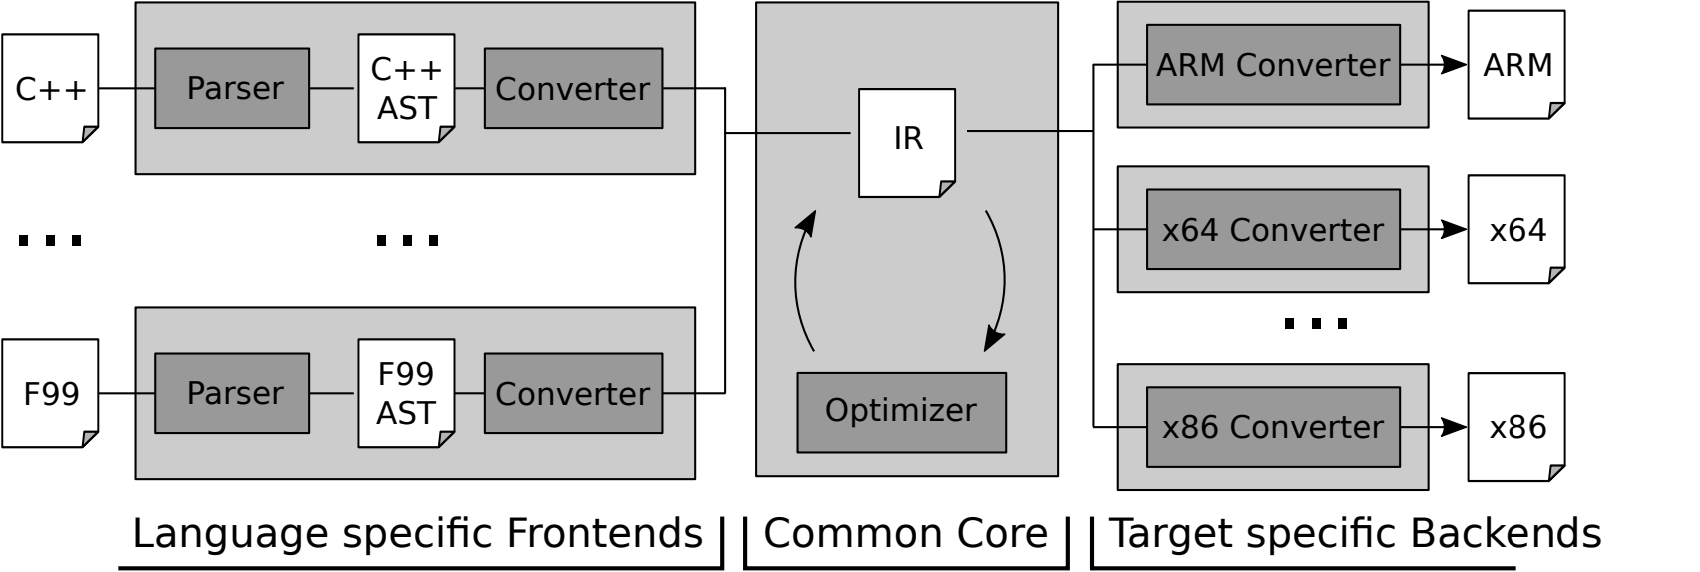
\includegraphics[width=\textwidth]{figures/generic_compiler_arch.png}
    \caption{A conceptual model of a retargetable compiler. Re-printed from \cite{Zangerl2018}}
    \label{fig:generic_compiler}
\end{figure}

To do so, they relied on two key insights: that these high-level languages were able to be transformed down to equivalent code in a subset of core imperative primitives that is still hardware-independent, and that this low-level intermediate representation (IR) contains enough information to perform most common optimizations.

Therefore, as seen in Figure~\ref{fig:generic_compiler}, we can conceptualize the retargetable compiler as a system consisting of three separate sets of modules:

\begin{itemize}
    \item Front-ends: these modules are responsible for parsing and checking the semantics of the source code, and then transforming it to the common intermediate language, which might imply compiling down language-specific features, such as monomorphization, dynamic dispatch, and so on. Usually, one front-end is implemented for each supported high-level language.
    \item Common core: this module is responsible for performing the bulk of the optimization steps, repeatedly transforming the program. Because these transformations are coded in terms of the intermediate representation, they can be re-used by each pair of source and target.
    \item Back-ends: Finally, the optimized code is processed to transform it to a code suitable for the final target, by performing target-specific tasks such as register allocation, instruction selection, linking according to the platform conventions, etc. These modules are usually implemented for each supported target.
\end{itemize}

Figure ~\ref{fig:llvm_arch} shows that LLVM's architecture aligns closely with this model. Support for each language or language family is implemented in separate front-ends (Clang for C/C++, rustc for Rust, the Julia compiler, etc.), which then generate code in the LLVM IR to be optimized by the LLVM optimizer, and finally a backend such as LLVM CodeGen \cite{LLVMCodeGen} can generate the output code (x86-64, Arm, WebAssembly), or another backend such as \textit{lli} \cite{LLVMDirectExecution} can directly interpret or JIT-compile the optimized IR.

\begin{figure}
    \centering
    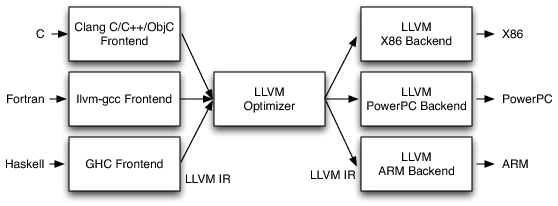
\includegraphics[width=\textwidth]{figures/llvm_arch.png}
    \caption{Diagram of LLVM compiler infrastructure's architecture. Reprinted from \cite{LattnerAOSA}}
    \label{fig:llvm_arch}
\end{figure}

Other compiler projects take a similar approach to their architecture. The GNU Compiler Collection uses several Intermediate Representations throughout the compilation process \cite{Novillo2004} - GENERIC, an abstract syntax tree representation; GIMPLE, a three-address-code representation; and a register transfer language - to simplify operations in different sections of the pipeline, and help modularize an otherwise monolithic architecture. Ongoing efforts \cite{GCCRearch} are being undertaken to further modularize this system into separate front-end, middle-end and back-end modules.
CompCert\cite{Leroy2009Compiler}, a formally verified compiler for the C programming language, also uses several intermediate representations to aid their goal of implementing and verifying each stage of the compilation process (see Figure ~\ref{fig:compcert_arch}).

\begin{figure}
    \centering
    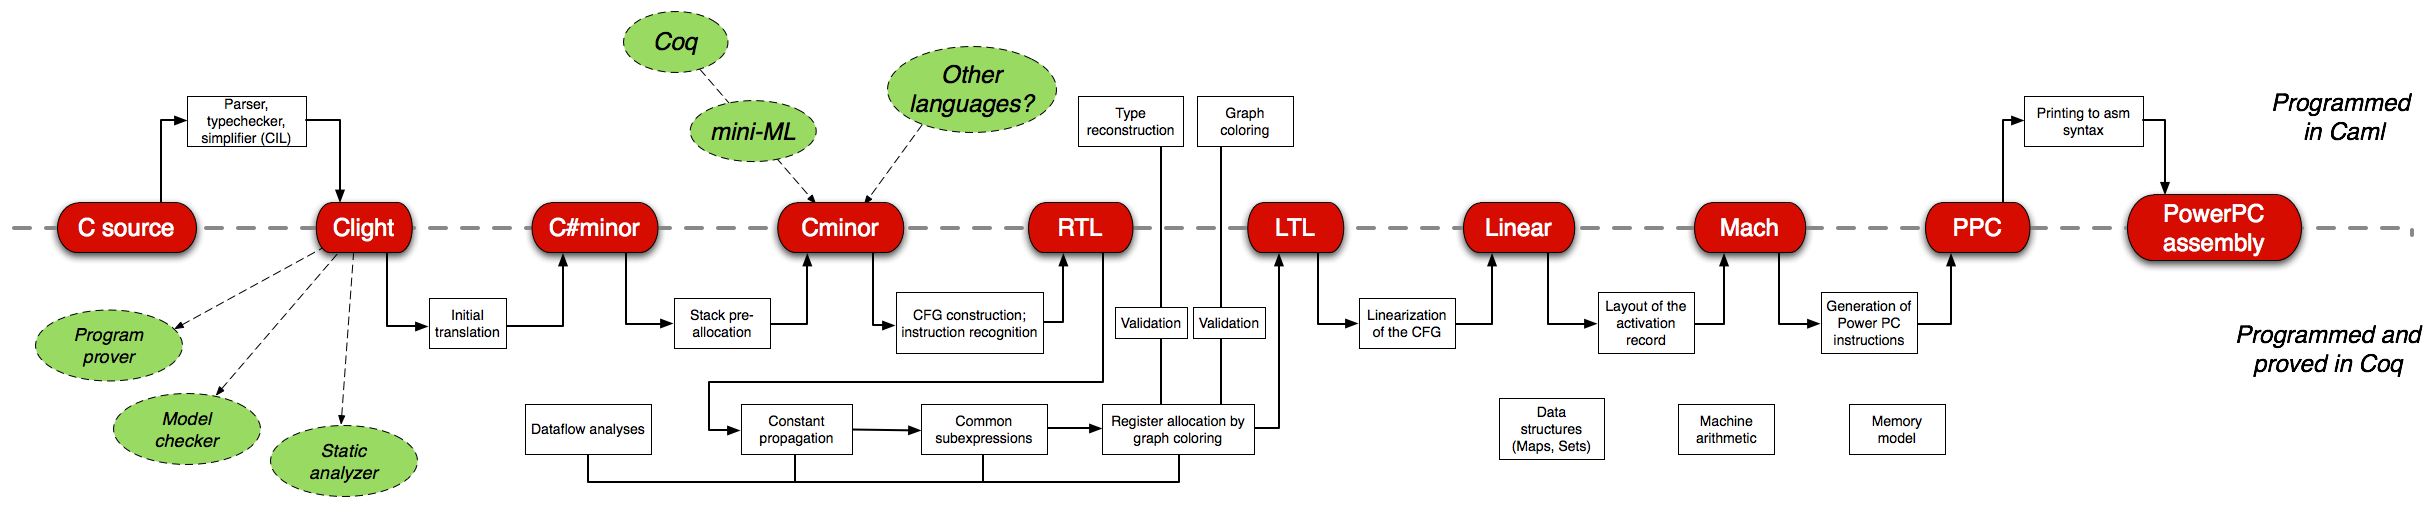
\includegraphics[width=\textwidth]{figures/compcert_arch.png}
    \caption{Diagram of CompCert's architecture. Reprinted from \cite{CompCertHome}}
    \label{fig:compcert_arch}
\end{figure}

\section{Optimization Techniques}

For the aims of our work, it proves useful to understand the kind of techniques that are commonly utilized to transform user-supplied codes into equivalent, yet more performant programs. This is done through analyzing the code and determining opportunities for transforming it into an optimized form, and performing those transformations, usually as a series of \textit{passes}, which yield a transformed version of the program.

We specifically wish to highlight two different aspects of the optimization process: the scope of the analyses, and the nature of the applied transformations.

\subsection{Scope of analysis for optimization}

Seeing as the first step of the optimization process is an analysis step, to determine which optimizations can be applied, we can distinguish optimizations by which scope the analysis is done.

The smallest scope is \textbf{local code analysis}. This analysis considers distinct instructions or small blocks of instructions. For example, let us consider the \textit{strength reduction} optimization. This optimization substitutes specific instances of complex instructions for equivalent but simpler, and therefore faster to execute, instructions. Consider the following two codes:

\begin{lstlisting}[language=C]
// prologue
// assume this variable exists and is set through an external interaction
int input_var;

// before strength reduction
int transformed_var = input_var * 4;

// after strength reduction
int transformed_var = input_var << 2;
\end{lstlisting}

The analysis is able to transform a multiplication by a power of two by an equivalent arithmetic shift instruction. Notice that, to perform this optimization, the analysis needs to just consider the one line of code, or a small block of instructions (load from memory, multiply with an immediate, store to memory). Therefore, it is \textit{local} in scope. In fact, this optimization can even be applied by linearly scanning the generated low-level code and replacing the instruction directly, in a process called \textit{peephole optimization}.

An intermediate scope at which analyses can be performed, and probably the most common one, is that of \textbf{global code analysis}\cite{Kildall1973}. This kind of analysis considers all visible code in a self-contained block, which usually corresponds to a function or procedure in the high-level language. Because such a scope might contain branching control and data-flow, stemming from the existence of loops and conditionals, these analyses rely on more advanced techniques, such as control and data-flow analysis\cite{Cytron1991}, logical induction of variables, etc, but in turn are able to deliver transformations that stem from the interaction between different blocks of instructions.

Some examples of this scope of analyses are:

\begin{itemize}
    \item Constant folding and propagation, or compile-time evaluation - this technique substitutes complex expressions whose arguments are only constants by the use of a single constant, that is yielded by performing the computation at the time of compilation.
    \item Common sub-expression elimination - this analysis detects expressions where a factor is repeatedly computed, and reworks the code to only compute it once, storing its value in a temporary variable to be reused.
    \item Loop unrolling - this analysis duplicates the body of a loop in the code, to perform fewer branches, which may improve instruction pipelining on the CPU.
    \item Dead code elimination - eliminates sections of the code which are unreachable, based on an analysis of the program's control flow.
    \item Some kinds of strength reduction, such as substituting the iterative computation of an arithmetic series by its direct computation, are only possible through global analyses, such as inductive variable analysis.
\end{itemize}

Even though this scope of analysis often suffices to perform many useful transformations, it carries the limitation that calls into other global scopes, such as calls to other functions, procedures, and units of compilation, are opaque, meaning that transformations which need information from several global scopes are impeded. To solve that issue, another scope of analysis is needed, \textbf{inter-procedural analysis}. On this scope, the interactions between different procedures are considered by analyses. Let us consider the following code as an example:

\begin{lstlisting}[language=C++]
template <type T>
class vector<T> {
    const T get(size_t i) const  {
        if (i < size) {
            return array[i];
        } else {
            throw Exception(/*...*/);
        }
    }

    size_t get_size() const {
        return size;
    }


    private:
    T* array;
    size_t size;
}

int main(void) {
    auto vec = new vector<int>();

    // initializing code here ...

    for (size_t i = 0; i < vec.get_size(); i++) {
        auto elem = vec.get(i);
        std::cout << elem * elem << '\n';
    }
}
\end{lstlisting}

In this code listing, we can intuit that there are several optimization opportunities that go unexploited unless we consider the interaction between both functions:

\begin{itemize}
    \item On line 26, a naïve call to the \textit{get\textunderscore{}size} function will involve multiple operations related to calling the function - saving to the stack a number of values whose registers might be overwritten, storing the parameters and the return instruction pointer in specific registers or stack positions, jumping to the subroutine, storing the return values in specific registers or stack positions, jumping back to the callee, restoring the values that were previously ejected from the registers, etc - even though the body of the function itself consists only of loading a number from a memory address. By using an inter-procedural analysis such as \textit{function inlining}, which duplicates the body of the called function inside the body of the caller, the compiler is able to remove such operations, yielding a simpler version of the code.
    \item While we can recognize that the loop header in line 26 and the branch in line 4 contain a duplicated condition check, simple global analysis in each procedure will not be able to detect such redundancy. However, an \textit{inter-procedural dead code elimination} analysis is able to do so, and remove the redundant check and associated unreachable code.
\end{itemize}

\subsection{Nature of transformations}

When considering which transformations can be applied in the context of optimizing codes, we distinguish the nature of the transformation, in relation to how it affects the performance of the code and the process of optimization itself.

Often, a transformation can itself be considered a \textbf{direct optimization}. The nature of these transformations is that they directly improve the performance of the transformed code. For example, strength reduction operations directly substitute computations for equivalent yet cheaper operations, directly improving the speed of the code. Likewise, constant propagation and folding allows computation to be shifted from run-time to compilation time, allowing expensive computations to be replaced by cheap loading of an immediate value.

On the other hand, some transformations might benefit the optimization process, regardless of their direct impact on the codes' performance. We term these \textbf{enabling transformations}. These transformations enable previously impossible optimizations, surfacing an emergent optimization property from the composition of different techniques\cite{Click1995}.

For example, function inlining may or may not impact positively the performance of the code\cite{Chen1993}, depending on the balance between the improved instruction pipelining, and the worsened program size, which may affect negatively the caching of the program's instructions. In any case, the extra information that the body of the inlined function provides may be instrumental in performing other analyses and transformations, such as dead code elimination, vectorization, or constant folding.

Another example of this phenomenon is constant folding and propagation. Besides directly reducing the amount of computation performed at run time, it may enable the compiler to prove that certain code paths are unreachable, aiding the process of dead code elimination.

Furthermore, some transformations, which are often called \textit{normalization} transformations, have the explicit goal of putting the analysed codes in a \textit{canonical form}, so that latter analyses have fewer edge cases to contend with, making the transformation code simpler and more maintainable. Examples of these include factoring complex computations into several temporary variables, or normalizing loop headers\cite{Gomes2021} e.g. so that they are always of the form \texttt{for (int i = 0; i < N; i++)}.

\section{Summary}

In this chapter, we have given an overview of important background concepts, for our work, namely by describing the three-stage architecture of modern optimizing compilers, and by categorizing the scope and nature of the analyses and transformations that they may perform on the programs they compile.
\chapter{Related Work}\label{chap:sota-lit}

To meet the challenges presented in Section ~\ref{sec:motivation}, several distinct approaches have been proposed and developed.

\section{Developments in IR-based optimization approaches}

\subsection{Mid-level Intermediate Representations}\label{sec:midlevel-ir}

As high-level languages have expanded their breadth to capture more semantic details, several compiler infrastructures have introduced their own IR between the high-level language, and AST, and the underlying optimizer, and its respective low-level IR.

These representations generally work on an intermediate level of abstraction, in which the set of syntactic constructs is restricted, and the semantic details of the language are encoded, as opposed to being eliminated in the process of lowering to a low-level IR.

Several of these approaches have been identified \cite{Lattner2021}:

\begin{itemize}
    \item The Rust compiler lowers the programs written in the language to their internal IR, MIR\cite{RustMirRfc}. This representation eliminates several syntax constructs to facilitate several analyses, such as liveness, death and reachibility checking, borrow checking (which implements Rust's static guarantees of memory safety), and guiding translation to the lower-level LLVM-IR.
    \item The Swift compiler lowers the programs to the Swift Intermediate Language (SIL) \cite{SwiftSIL}, which they use to provide the following analyses: "A set of guaranteed high-level optimizations [...]. Diagnostic dataflow analysis passes that enforce Swift language requirements [...]. High-level optimization passes [...]. A stable distribution format that can be used to distribute 'fragile' inlineable or generic code with Swift library modules, to be optimized into client binaries."
    \item The Julia compiler lowers the programs to a SSA-form representation \cite{JuliaIR} after performing macro inlining and other syntax simplification tasks, in order to perform middle-end optimization tasks.
\end{itemize}

While the intermediate level of abstraction might be appropriate for some optimizations, this approach is limited by several factors.

Firstly, it still ties the optimization work to a single compiler implementation: whereas these languages have had their effort mostly concentrated on a single implementation (Swift compiler, \textit{rustc}, and the Julia compiler) and so are able to mitigate this disadvantage, other source languages, such as C and C++, have multiple compiler implementations, where this approach suffers from a fragmentation of effort.

Moreover, this approach continues to necessitate a lowering of the level of abstraction, which might impede optimization efforts that depend on high-level details of the programming language. This effect is exacerbated when considering the use cases of finding optimizations for codes that make use of eDSLs or libraries \cite{Zangerl2018}.

\subsection{MLIR: Declarative approach to defining and optimizing a Multi-Level Intermediate Representation}

Another recent contribution in this space is MLIR \cite{Lattner2021}. This extension of the LLVM representation aims to deal with several deficiencies of that system's approach to compilation, namely shortcomings in dealing with heterogeneous targets and non-scalar data.

To that end, it formalizes a system of intermediate representation with the following characteristics:

\begin{itemize}
    \item Ability to capture multiple levels of abstraction through the use of nested blocks of operations, and the use of attributes to capture semantic details of tagged code regions.
    \item Separation of concerns between different translation passes through the definition of dialects, static traits and dynamic interfaces.
    \item Ability to define schemas for non-scalar data.
    \item Declarative approach to defining code transformations, including the ability to progressively and partially lower the abstraction level of code regions.
\end{itemize}

A practical example of this approach is the recently proposed Clang Intermediate Representation \cite{CirRfc} (CIR). This representation leverages MLIR's ability to define dialects and transformations within and between them to provide an intermediate language that does not necessarily rely on the syntactic constructs of the C and C++ languages, but allows important semantic concepts from these languages to be abstractly represented and reasoned about in analyses, before being morphed into other, and lower-level, IR dialects.

While this approach might prove valuable in its stated goal of generalizing and driving a wide goal of compiler projects, the generic nature of the representation may worsen the ergonomics of developing code transformations. In particular, the transformation implementer must learn the semantics of the IR representation, which is constructed to support the semantics of the language but not derived from it, and how to perform transformations on it. In the case of MLIR, the implementer must, depending on the specifics of their transformation, implement the transformation in terms of an external DSL and Python bindings, or even may need to write out their transformation imperatively, using a C++ template-based system.

In comparison, using source-to-source compilation allows us to provide a simpler development experience to users. By relying on the structure and semantics of widely supported high-level languages (C and C++), we are able to support a wide range of targets and assure the users that if they are able to implement the transformation on high-level code, they will be able to automate it. By relying on source-code normalization and simplification passes, we are able to provide a representation that is derived from the high-level language by subtraction, which can more immediately be understood (it is "just a simple C/C++"). Not only that, by providing an compiler interface embedded on, or embedding, an extremely popular and easy-to-use language such as Javascript, we are able to provide the optimization developers-to-be with a more ergonomic experience.

\section{C Intermediate Language: Source-to-Source normalization of C code}

Another work that is particularly relevant for this dissertation is the C Intermediate Language \cite{Necula2002}. This project is similar to, and can be in some ways considered to be a precursor of, our work, as it similarly recognizes that the C language has a wealth of complex constructs hampering a straightforward analysis process of source programs.

To tackle this issue, it constructs a high-level representation that preserves most semantic aspects of the C source code, but simplifies several aspects of the language, including removing redundant constructs and syntactic sugar, making implicit casts explicit, and separating value evaluation, side-effect creation, and control-flow changes. It also incorporates a Control Flow Graph into the representation to make analyses relying on it simpler. After converting to this representation, it applies any transformations that the user has specified, using an embedded DSL in OCaml, and outputs the transformed program in C.

As close as this approach may be to our work, there are still some different trade-offs between this approach and ours:

\begin{itemize}
    \item This approach still works by constructing a new representation that, while mapping closely to the source language, still is separate from it. While this allows for a significant transfer of domain knowledge compared to other IR-based approaches, it still is not as close to the source language as we desired. In comparison, our AST-based approach, which only subtracts elements that are deemed too complex, keeps a more faithful representation of the original program.
    \item The language proposed by the authors eliminate some features, such as some kind of syntactic sugars (\verb|->|) or scoped variable declarations, that we consider to be useful enough and simple enough that they do not hamper the analysis of the language, while departing from the original program.
    \item The front-end parser for the language is rather limited, only supporting ANSI C with some GNU and MSVC extensions. While this is understandable when considering the age of the tool, it stands in contrast with Clava, which is able to use Clang's frontend tooling to support codes written not only in C, but also C++ and OpenCL, evolving to support more recent features of the language as Clang evolves to support them too.
    \item When implementing further transformations, CIL requires them to be written using a limited interface based on OCaml and using only a visitor pattern. In contrast, the LARA environment that Clava uses allows full access, including imperative modification if needed, to the program's AST, using a widely-used host language (Javascript).
    \item While CIL does preliminary analysis to present a unified CFG and AST representation of the program, this needlessly complicates reasoning about program when such analysis is not required. In the Clava standard library, we implement normalization and control-flow analysis separately, improving separation of concerns between these two tasks.
\end{itemize}

\section{C--: Reduced C-language Subset as Compilation Target}

Another set of authors that historically proposed the use of a reduced subset of C as a language to be used by compilers is Peyton Jones, Ramsey, and Reig, with C-- \cite{Jones1999}.

In their work, the authors identify several limitations encountered by using C as a portable assembly language to be targeted by compiler front-ends for other abstract programming languages. Specifically, they mention the lack of support of continuations, multiple return in registers, control of the stack framing and calling conventions, among other deficiencies as severely limiting to implementing functional languages like Haskell, ML, or Scheme.

To solve this issue, they propose a language that at first sight looks like a simplified version of C, but is not a proper subset. They define abstractions to control a number of lower-level behaviors, such as precise control over static data layout, and stack-less jumps to implement continuations or perform tail call elimination.

While there is stand-alone value in this approach for its purported use case of providing a portable target to implement high-level languages, though a fair comparison with more recent contributions in IRs \cite{Lattner2004} is warranted, this approach does not meet our particular use case.

With our contribution, our goal is to support an optimization use case for compiler-independent analysis and transformation of C and C++ programs, not programs in other languages. That means that it is more ergonomic to provide a representation that captures a proper subset of our source languages, and we do not feel the need to break the confines of the C and C++ languages as they are specified.

\section{Formally-verified optimization techniques for certified compilers}

In the context of certified compiler implementation, several recent contributions have aimed to implement formally-verified optimizations for the CompCert project:

\begin{itemize}
    \item Tristan and Leroy, 2009 \cite{Tristan2009} implement and formally verify a Lazy Code Motion optimization pass.
    \item Barthe et al, 2014 \cite{Barthe2014} contribute a formally-verified middle-end that adopts an SSA-form intermediate representation, which simplifies the implementation of further optimizations.
\end{itemize}

These two contributions have in common the use of a combined technique for implementing verified compilers. Specifically, the respective authors follow a process where they implement the optimization pass using an unverified algorithm, for performance purposes, and introduce a subsequent verification pass where a formally-verified validator program checks the correctness of the transformation.

Another contribution in this space is a formally-verified implementation of a global common sub-expression elimination and loop-invariant code motion pass \cite{Monniaux2021}.

These contributions prove that, with enough effort, it might be possible to formally verify and implement a large breadth of optimization techniques, but several concerns remain unaddressed:

\begin{itemize}
    \item The optimization work is still tied to a specific compiler. This aspect is exacerbated by the consideration that other compilers' models might not be formally specified or validated to the same extent, and that the presence of differing abstractions between compilers will now entail not only the need to adapt the implementation, but also the validation step.
    \item Although we consider these contributions a good first step in proving that it is possible for certified compilers to be enhanced in their optimization abilities, there are other reasons that might impede their modification by users and researchers, such as their being proprietary or other impeding circumstances.
    \item In some cases, namely during prototyping work, it might be desirable to work with a single, high-level abstraction, whereas the process of verification necessitates multiple, more detailed formal constructs.
\end{itemize}

For this reason, we consider that the use of source-to-source compilation, followed by the use of a certified compiler for the final compilation step, might be a good middle-of-the-road alternative to provide a degree of safety and simultaneously allow for research into new optimization techniques.

\section{Summary}

In this chapter we have given an overview of recent related contributions to our work. We found that there have been efforts in providing more flexibility to IR-based approaches and in formally-verifying optimization passes for certified compilers.

We reached the conclusion that there is space to push further with a source-to-source compilation approach to analysis and transformation, which we detail in Chapter ~\ref{chap:gen_approach}.
\chapter{General Approach}\label{chap:gen_approach}

To fulfill our objective of providing an environment where program analysis and optimization research for C and C++ is faster and more ergonomic, we focused on the following general approach:

\begin{enumerate}
    \item Define a language subset where program analyses need to account for fewer primitives, constructs and edge cases.
    \item Implement a series of transformations that normalize a given program to only use said language subset.
    \item Target a specific optimization to be evaluated.
    \item Implement the optimization as a transformation to be applied to the code.
    \item Apply the normalization and optimization passes on sample programs and benchmarks.
    \item Compile with standard toolchains and evaluate the performance of the optimization.
\end{enumerate}

\section{Architecture}

\begin{figure}
    \centering
    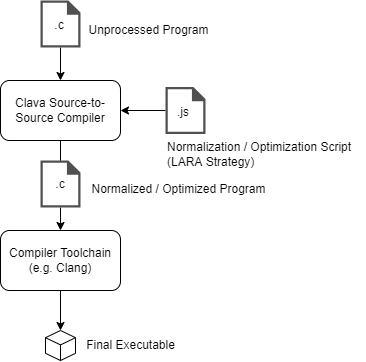
\includegraphics[width=0.5\textwidth]{figures/general_architecture.png}
    \caption{Diagram showing the overall architecture of the compilation system.}
    \label{fig:general_arch}
\end{figure}

We chose to simplify the architecture of our system as much as possible, by using the source-to-source compiler, Clava, to output source code files that can be used with a pre-existing standard compilation toolchain, such as LLVM, instead of imposing a specific choice of compiler. Figure \ref{fig:general_arch} shows the general architecture of the system as described.

Firstly, we implement the normalization and optimization passes using the Clava source-to-source compiler. Clava is fully scriptable in Javascript, using an embedded DSL. As described in Figure \ref{fig:clava_arch}, Clava parses the input C or C++ programs using Clang's libtooling library, and generates an AST representation for them. This representation is then automatically converted to an AST for use inside the LARA Framework's Javascript environment, where scripts written in Javascript can manipulate the AST at will. At this stage, we run a series of transformations to simplify and optimize the AST representation of the program, and output the transformed version of the program in the source language.

Afterwards, we are able to use the transformed program as input of a compilation toolchain of choice. This allows us to provide the maximum portability for the final build step of our compilation process, by allowing us to choose a compiler that is the most appropriate for any given use case. If the target of our compilation is a general-purpose computer running a mainstream operating system, we are able to use any popular compiler, such as the Clang compiler, the GCC compiler, or the MSVC compiler, as the backend for our process. Furthermore, Clava already provides an integration with CMake, making this process easier for existing projects. If, on the other hand, we need to use a certified compiler, such as CompCert, or a compiler that is specific to an specialized use case, such as automotive or embedded systems development, we can still use Clava as the front-end. This is only possible because we are using the source language as the target of our optimizations, yielding a program that is at least as portable as the original program. Besides that, the Clava compiler and the LARA Framework are both developed in-house at FEUP's SPeCS laboratory, which allowed us to leverage existing expertise with the tool to quickly prototype our research, and quickly communicate and fix any tooling flaws that were identified, which made it a natural choice over other source-to-source compilation systems.

\begin{figure}
    \centering
    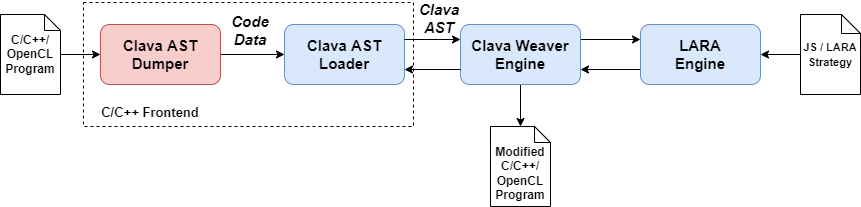
\includegraphics[width=\textwidth]{figures/clava_arch.png}
    \caption{Diagram of Clava's architecture, in relation to the LARA framework. Adapted from \cite{Bispo2020}.}
    \label{fig:clava_arch}
\end{figure}

\section{Organizing Analyses and Transformations Effectively in Clava}

Another question that we faced was understanding how the analyses and transformations that we aimed to implement could be organized to maximize the ease of development and showcase the ergonomy benefits of our approach.

Firstly, it is useful to revisit the goals set out in the introduction of this work. As mentioned then, one of the goals for the transformations provided is that they should be automatic. This means that we cannot, for the most part, rely on the developer to indicate which transformations should be transformed in which parts of the code. To fulfill that goal, we relied on the already existing notion of \textit{transformation passes}, which is present in most compilers. This abstraction posits that the transformations that we aim to perform on the code can be modelled as a sequence of discrete transformations to be applied to the program. A pass will, in principle, be composed of two separate elements. First, an analysis must be performed, usually resorting to structural pattern matching on the program, to identify cases where a certain transformation may be applied profitably. Afterwards, the transformation is applied to the identified program fragments, modifying its structure and yielding a new code for that fragment that meets the compiler developers' goals of improving non-functional aspects of the code or enabling further transformations, while maintaining the function of the existing program. Because of the structural nature of these analyses, the use of an AST-based compiler provides an interesting advantage for implementing them: the variety of primitives present in the source language and associated AST allows many structural elements to be explicitly modelled, reducing the need to perform complex analyses to re-surface those details from a lower-level representation.

We introduced, therefore, to the LARA framework the Pass abstraction, which is responsible for, from any given node of an AST, finding the descendants to which a given transformation can be applied and applying the desired transformation to the relevant nodes, yielding back to the main script statistics and error diagnostics for development purposes, as well as implementation specific details such as whether the program should be re-parsed to deal with inserted literal code. To use this abstraction, the researcher only needs to implement a predicate establishing whether a specific node in the AST is a candidate to be transformed in that pass, and a function that performs said transformation, and the abstract implementation can be responsible for visiting the matching nodes in the AST and transforming it.

Finally, to support the goal of providing a frictionless environment, we implemented our language normalization algorithm as part of the Clava standard library.

\section{Validation Case Study: Function Inlining}

After having defined our normalized language subset and implemented the transformations to obtain it, we validate the approach by implementing a sample code optimization transformation - in this case, we chose function inlining. The choice of transformation was made based on three main factors: the first factor we considered was the ease of translating the model of the transformation in terms of a source-to-source transformation. Inlining proved an interesting candidate under this factor because, in the optimal case of isolated calls, it can trivially be implemented by copying the code of the inlined function into the body of the function that calls it. The second factor we considered was choosing a transformation whose implementation was tangibly eased by the preceding code normalization steps. In the case of inlining, the possibility of calling functions within nested expressions, which was removed by our code normalization steps, impeded a straightforward implementation of the optimization, whereas normalized code targeting our subset has clearly delineated calls, allowing the transformation to be applicable in more cases. Finally, the final factor that we considered was that the optimization that we would implement should provide a clear non-functional improvement to the final program. In the case of function inlining, we theorized, based on previous experiments and literature \cite{Chen1993}, that the transformation would provide clear performance improvements when inlining a small function in a hot section of the caller, such as inside a loop, by removing unnecessary branching and improving instruction cache locality.

In terms of a strategy for evaluation, we opted to evaluate our case study along two axes. The first axis is ergonomics. In particular, we tested two versions of an inliner transformation and evaluated whether the normalization steps allowed the inlining to operate in more cases than previously allowed. The second axis is the quantifiable effect on runtime performance of code processed with our transformations. We tested both synthetic micro-benchmarks created by us to illustrate ideal cases of applicability for function inlining, and a more general suite, NAS, to exercise our transformed code and provide a better point of comparison with related work.

\section{Summary}

In this chapter, we discussed the general approach that our solution takes to solve the problem of providing functional and ergonomic support for code optimization research for C and C++. Particularly, we enumerate the main tenets of our approach and present the general architecture of our compilation system, accompanied by a high-level discussion of the trade-offs that led us to that choice. This is followed by a discussion of the logical organization of the proposed techniques' implementation, and by a brief discussion of our approach to validating and evaluating our work.

\chapter{A Normalized Subset of the C and C++ Languages}\label{chap:subset}

As we explored earlier in this work, two factors predominate in providing researchers and developers with a powerful and ergonomic program optimization platform.

The first, the tooling's ability to provide simple, yet powerful abstractions for querying and manipulating the programs, is arguably tackled, even if not yet completely, by the use of Clava, with its simple model and straightforward scripting in a high-level language.

However, the other predominant aspect, one that goes under-appreciated, is ensuring that the level of abstraction of the representation used is appropriate for the task at hand. This requires balancing parsimony - making sure that only the language elements that are needed to represent the domain are exposed, and no more - and expressiveness - exposing a set of language elements that is rich enough to represent the domain in a natural and concise way. The balance between the two factors naturally depends on the task. Let us consider two  examples that typify opposite ends of this balance.

\begin{itemize}
    \item A refactoring tool will find itself needing an extremely expressive intermediate representation. This stems from the overwhelming need to preserve most of the syntactic structure of the original program, compared to the relatively local kinds of changes that will be performed (such as renaming the occurrences of a variable, or extracting a method out). In extreme cases, even spacing, line breaks and indentation must be preserved, so corresponding elements must be present in the internal language.
    \item On the other hand, the middle and back-ends of a standard compilers may admit and use a much more restricted set of elements in their intermediate representation. This occurs because the target language is not meant for human consumption and is itself quite parsimonious, and because simpler languages are often easier to statically analyze, since structural pattern matching must account for a smaller set of elements and their combinations.
\end{itemize}

By analysing the use case that we tackle: supporting ergonomic, automatic yet inspectable research and implementation of program optimization, we are able to establish a set of principles to navigate this trade-off, and to present a \textit{normalized} or \textit{canonical} subset of the C and C++ languages to use as our intermediate representation.

This chapter presents these underpinning principles, and contributes a set of transformations that may be applied to reach our normalized subset.

\section{Simplified, but structured, control flow}\label{sec:subset-control-flow}

The first set of complexities that were tackled is the diverse set of control flow constructs. Control flow in C and C++ is performed by using several different statements, which can be categorized further into several categories:

\begin{enumerate}
    \item Selection statements
    \item Iteration statements
    \item Unstructured control flow statements
\end{enumerate}

For each of these categories, we considered whether the corresponding statements could be replaced with a set of patterns using fewer primitives, while rejecting the goal of replacing structured control flow statements with equivalent patterns made of unstructured control flow statements.

\subsection{Selection statements}

C and C++ use the if-statement as the main pattern for structured selection control flows. This statement takes an expression as a condition, and, depending on it evaluating to a non-zero (\textit{truthy}) or zero (\textit{falsy}) value, it will execute the statement contained in a respective statement (termed as the \textit{then} or \textit{else} branch of the statement). We consider this statement the main candidate for being the target of normalization of other selection statements.

The language allows several expressive liberties to be taken when using this statement, so Clava already performed several normalization steps for this statement. Specifically:

\begin{itemize}
    \item A branch of this statement could be a single statement, or a compound statement (a scope, denoted by the use of curly brackets around one or more inner statements). Clava automatically inserts a scope around single statements.
    \item The else branch is optional. In that case, no statement would be executed if the condition was falsy. Clava automatically inserts an empty scope for that branch.
\end{itemize}

This means that a code like:

\begin{lstlisting}[language=C]
if (condition) singleStatement();
\end{lstlisting}

Is transformed into the code:

\begin{lstlisting}[language=C]
if (condition) {
  singleStatement();
} else {}
\end{lstlisting}

Furthermore, the ternary operator can be considered a selection statement as well. As with the if-statement, this operator takes an expression as a condition, and evaluates to different expressions depending on whether the condition evaluates to a truthy or falsy value.

We aimed to rewrite this operator in terms of the if statement, and so implemented the transformation \verb|clava.code.SimplifyTernaryOp| to do so automatically. Leading the following code:

\begin{lstlisting}[language=C]
condition ? trueExpr : falseExpr;

a_type result = condition ? trueExpr : falseExpr;
\end{lstlisting}

To be transformed into:

\begin{lstlisting}[language=C]
if (condition) {
  trueExpr;
} else {
  falseExpr;
}

a_type result;
if (condition) {
  result = trueExpr;
} else {
  result = falseExpr;
}
\end{lstlisting}

This transformation furthermore requires that non-linear control flow in evaluated expressions is performed explicitly, as detailed in \ref{sec:subset-expressions}, so as to have ternary operators be placed in top-level statements or as the right hand side of a top-level assignment.

Finally, we must consider the existence of the switch (case) statement, which evaluates a condition and jumps to an execution path based not on the truth value of a condition, but by comparing it to a set of values (the cases of the statement). However, this statement, in C and C++, does not exhibit structured control flow by default, since in the absence of a break statement, the flow of execution falls through to the code path of subsequent cases in the code. It is however possible to devise a transformation that, based on analysing the existence or nonexistence of break statements and using code duplication, could guarantee structured control flow in these cases, transforming code such as:

\begin{lstlisting}
switch (cond) {
  case 1:
    stmt1_1;
    stmt1_2;
  case 2:
    stmt2;
    break;
  case 3:
    stmt3;
}
\end{lstlisting}

Into code like:

\begin{lstlisting}
switch (cond) {
  case 1: {
    stmt1_1;
    stmt1_2;
    stmt2;
    break;
  }
  case 2: {
    stmt2;
    break;
  }
  case 3: {
    stmt3;
    break;
  }
}
\end{lstlisting}

allowing the switch statement to be subsequently transformed into a chain of if statements:

\begin{lstlisting}
if (cond == 1) {
  stmt1_1;
  stmt1_2;
  stmt2;
} else if (cond == 2) {
  stmt2;
} else if (cond == 3) {
  stmt3;
}
\end{lstlisting}

The main factor that complicates this transformation is that there is no guarantee that the control flow in a switch statement is structured. For example, one could have case labels in between components of an if statement, or a Duff's device \cite{Duff1988}, or declarations that are unreachable for a label but reachable code that nevertheless uses said declarations. Therefore, it was infeasible, at least for the scope of this work, to devise a general transformation for this case. We also decided to de-prioritize work on a restricted version of it, so no attempt was made at such implementation.

\subsection{Iteration statements}\label{sec:subset-iteration}

Iteration statements are statements where a condition is repeatedly evaluated, and a set of statements are executed as long as the condition holds. The C and C++ languages define four types of statement to perform this control flow: the while statement, the do-while statement, the traditional (three statement) for statement, and the range or iterator-based for statement (for-each statement, in our parlance).

While these statements could be rewritten in terms of selection statements and unconditional jumps, the pattern of iteration is important enough to warrant explicit expression, and at least one of the iteration statements should be kept. Thus we chose to keep as a primitive the while statement, which is the conceptually simpler of the four. The while statement evaluates the condition at the \textbf{beginning} of each iteration and executes the body if the condition holds true.

The other conceptually simple statement is the do-while statement. The do-while statement evaluates the condition at the \textbf{end} of each iteration, and so is guaranteed to execute \textit{at least one} iteration.

The processes for transforming a while statement into a do-while statement and vice-versa are well known. To transform a while statement into a do-while statement we would perform a \textit{loop inversion}: replace the while statement with a do-while statement, and wrap it in an if statement, duplicating the condition. This inversion often proves to be worthwhile in terms of performance, since it reduces the number of branches, which predominates over the duplicated code to calculate the condition.

However, we find that while statements are generally more used and better understood, so we implemented instead the transformation \verb|DoToWhileStmt|, which transforms a do-while statement to a while statement by peeling the first iteration in a separate scope before the transformed loop, transforming code such as:

\begin{lstlisting}
stmt0;
do {
  stmt1;
  stmt2;
} while(cond);
\end{lstlisting}

Into code like:

\begin{lstlisting}
stmt0;
{
  stmt1;
  stmt2;
}
while(cond) {
  stmt1;
  stmt2;
}
\end{lstlisting}

While this transformation results in more duplicated code, we believe that its expected infrequency compared to the reverse transformation makes it more desirable.

The next element to consider is the for statement. This statement allows the user to concisely define a canonical loop by having the usual steps of it (declaring the inductive variable, expressing the loop condition, and stepping the inductive variable) all present in the loop header. However, to maintain our desirable degree of parsimony, we implemented the \verb|ForToWhileStmt| transformation, which extracts out the initialization and step sub-statements and transforms the for statement into a while statement, turning code like:

\begin{lstlisting}
for (init; cond; step) {
  stmt1;
  stmt2;
}
\end{lstlisting}

Into:

\begin{lstlisting}
{
  init;
  while (cond) {
    stmt1;
    stmt2;
    
    step;
  }
}
\end{lstlisting}

Finally, we considered the C++-only 'range-based for statement', or for-each statement for short. This statement can be converted in a straight-forward manner to a for statement, according to the C++ standard:

\begin{quote}
The range-based for statement

\verb|for (init-statement for-range-declaration : for-range-initializer)|
\verb|  statement|

is equivalent to
\begin{verbatim}
{
  init-statement
  auto &&range = for-range-initializer ;
  auto begin = begin-expr ;
  auto end = end-expr ;
  for ( ; begin != end ; ++begin ) {
    for-range-declaration = * begin ;
    statement
  }
}
\end{verbatim}
\end{quote}

Following that, it could be further rewritten in terms of a while statement. We did not implement this transformation, since we considered it to be of low priority in a prototypical implementation.

\subsection{Unstructured control flow}

The last category of statements that we considered were unstructured control flow statements:

\begin{itemize}
    \item Break statements
    \item Continue statements
    \item Early return statements
    \item Exception throwing and catching
    \item Long jumps
    \item Go-to statements
\end{itemize}

These statements, in the general case, cannot be converted to equivalent structured statements without introducing meaningfully complex code changes and/or auxiliary variables, so we decided against implementing transformations to remove them. Two exceptions were made against this decision.

Firstly, in the case where for statements were converted to while statements, it was necessary to transform continue statements into equivalent go-to statements to a label before the step expression at the end of the loop.

Secondly, a transformation to remove early returns from a function, by introducing unconditional jumps to the end of a function and the use of an auxiliary variable, was developed, for use in specific applications (such as function inlining).

\section{Explicit side-effects and transfers of control flow in expression evaluation}\label{sec:subset-expressions}

C and C++ allow the building of arbitrarily complex expressions to be evaluated during execution, expressions which may contain elements in their construction that perform side-effects or transfer control flow in some way.

Some examples of this complexity may include divergent control flow in evaluation, such as when using ternary operators, side-effects during expression evaluation, such as when evaluating assignments and unary increment and decrement operators, and potentially interprocedural jumps, such as when evaluating a call or a throw.

In many situations, when performing analyses, it is useful to separate these complexities from the comparatively mundane calculations that may be performed around them.

Furthermore, we found that, when performing some transformations, such as function call inlining, there were cases where we would need to place several statements in a place that only accepted a single expression, and so it would be useful to separate the complex steps of a certain expression's evaluation from its use, in order to simplify implementation.

Therefore, we aimed to restrict the expression syntax to a more manageable set of elements. Specifically, we decided that any use of an expression (such as in a call parameter or in a header of a selection or iteration statement) could only be made with an immediate or an existing variable, and that the evaluation of any complex expression ought to be simplified by using one or more temporary variables, according to the following rules - the rvalue of a variable assignment can be:

\begin{itemize}
    \item An immediate or an existing variable.
    \item One or more unary operators applied in succession to an immediate or an existing variable. Unary decrement and increment operators are not allowed.
    \item A binary operator, whose arguments are an immediate, an existing variable, or another binary operator, to which this restriction on allowed arguments applies recursively. Assignment operators are not allowed.
    \item An interprocedural call, whose arguments can only be an immediate or an existing variable.
\end{itemize}

In general, these restrictions should be understood to adhere to the principle that \textit{expressions should pertain only to combinations of pre-existing and primitive values}. Other concerns should be dealt with externally to expression evaluation.

Of course, these restrictions imply that a range of valid expressions must be rewritten using our restricted set of constructs. The following subsections detail such cases, and how they were rewritten.

Other expressions need only to be decomposed. In those cases, we insert temporary variables to contain the intermediate results of those expressions' evaluation.

After this process of transformation and decomposition, we are left with a sequence of statements to be placed preceding to any place the expression is evaluated in, a new value for the expression, and a sequence of statements to be placed after the evaluation\footnotemark. These statements might be repeatedly inserted, depending on the control flow of the program (for example, in a while statement, the preceding statements will be inserted before the loop and at the end of each iteration, and the succeeding statements will be placed at the beginning of each iteration and after the loop, coinciding with the occasions where the loop condition is evaluated). \footnotetext{Strictly speaking, there is not a specific total order of evaluation, as the standards do not mandate a general order of evaluation, unless an operator with more specific semantics introduces such an order. These operators are known to introduce \textit{sequence points} into the program evaluation. Examples of such operators are: the comma operator, short-circuiting union and intersection operators, ternary operators, function calls, among others. In practice, we must serialize the order of evaluation anyway, since the program source is sequential by nature, so we serialize the expression tree left-to-right, post-order.}

\subsection{Explicit side-effect evaluation}

There are several expressions in C and C++ that can also effect changes on the global state. These expressions, while useful when writing expressive, high-level code, can complicate reasoning about the program automatically, since, for a single expression, both value production and side-effects must be tracked. Therefore we aim to rewrite these expressions to separate value computation and side-effect application.

The first kind of expressions that needed to be rewritten were the ones that performed side-effects on the variables they were operating on. These were assignment operators and unary increment and decrement operators. These operators, while returning a value, simultaneously mutate a variable. Separating this mutation is useful to allow analyses to reason about the mutation separately, and to be able to assume that expression evaluation is a pure computation.

Therefore, we devised transformations to insert a separate statement performing the mutation, and to reference the results of the mutation explicitly, according to the semantics of each operator:

\begin{itemize}
    \item When evaluating an assignment operation, the assignment will be performed in a previous statement, and the lvalue of the assignment will be subsequently used in the computed expression.
    \item When evaluating a pre-increment or pre-decrement unary operator, the increment or decrement will be inserted before the expression evaluation, and the target will be used in the computed expression.
    \item When evaluating a post-increment or post-decrement unary operator, the target will be used in the computed expression, and the operation will be inserted as a subsequent statement.
\end{itemize}

This means that code like:

\begin{lstlisting}
int a = 1;
int i = 2;
int j = 3;

int b = (a += i++ + ++j);
\end{lstlisting}

Will be rewritten to:

\begin{lstlisting}
int a = 1;
int i = 2;
int j = 3;

++j;
a += i + j;
int b = a;
i++;
\end{lstlisting}

Afterwards, the isolated unary increment and decrement operators can safely be rewritten to a simple assignment with a sum.

\subsection{Explicit transfers and divergences in control flow}

We also strive to make complex control flow more explicit. 

Firstly, calls are isolated from other elements of the expression:

\begin{lstlisting}
int a = f(b, g(c, d);

// becomes

int temp0 = g(c, d);
int a = f(b, temp0);
\end{lstlisting}

Secondly, ternary operators are completely removed and rewritten in terms of an if-statement, after they are separated from the rest of the expression evaluation:

\begin{lstlisting}
int a = conditionA ? (conditionB ? expr1 : expr2) : expr3;

// becomes

int a;
if (conditionA) {
  if (conditionB) {
    a = expr1;
  } else {
    a = expr2;
  }
} else {
  a = expr3;
}
\end{lstlisting}

Another relevant transformation, that was not implemented and is left as future work, is rewriting short-circuiting boolean operators with if statements, so as to preserve the sequencing and conditional execution properties of the operator when the operators are decomposed. This would mean that a statement such as:

\begin{lstlisting}
bool condition;
condition = (expr1 && expr2) || (expr3 && expr4);
\end{lstlisting}

Would be rewritten not as:

\begin{lstlisting}
bool condition;

bool temp1;
temp1 = expr1;
// semantic error: executes side-effects of `expr2` when `expr1` evaluates to false
bool temp2;
temp2 = expr2;
bool temp1and2;
temp1and2 = temp1 && temp2;

// semantic error: executes side-effects of `expr3 && expr4` when `expr1 && expr2` evaluates to true
bool temp3;
temp3 = expr3;
// semantic error: executes side-effects of `expr4` when `expr3` evaluates to false
bool temp4;
temp4 = expr4;
temp3and4 = temp3 && temp4;

condition = temp1and2 || temp3and4;
\end{lstlisting}

But as:

\begin{lstlisting}
bool condition;
{
  bool tempUnion;
  {
    bool temp1and2;
    {
      temp1and2 = expr1;
    }
    if (temp1and2) {
      // correct: only executes side-effects of `expr2` when `expr1` evaluates to true
      temp1and2 = expr2;
    }
    tempUnion = temp1and2;
  }
  if (!tempUnion) {
    // correct: only executes side-effects of `expr3 && expr4` when `expr1 && expr2` evaluates to false
    bool temp3and4;
    {
      temp3and4 = expr3;
    }
    if (temp3and4) {
      // correct: only executes side-effects of `expr4` when `expr3` evaluates to true
      temp3and4 = expr4;
    }
    tempUnion = temp3and4;
  }
  condition = tempUnion;
}
\end{lstlisting}

A final transformation that was left unimplemented was removing the comma operator, which would transform code like:

\begin{lstlisting}
// void side_effect(int *n);
// int arg;
int n;
n = side_effect(&arg), arg;
\end{lstlisting}

Into:

\begin{lstlisting}
// void side_effect(int *n);
// int arg;
int n;
side_effect(&arg);
n = arg;
\end{lstlisting}

\section{Overall simplification of the language and removal of superfluous elements}

Besides the two kinds of simplification detailed in the two previous sections, we defined a further set of simplifications to be made to the language. They consist of rote substitutions of convenience operators for their more verbose primitive versions, and other simple transformations. These include:

\begin{itemize}
    \item Breaking up variable declaration statements into several statements, to ensure that only one variable is declared in each statement.
    \item Separating variable initialization from variable declaration, by placing the initial value in a separate assignment statement.
    \item Removing complex assignment operators, by replacing with assignments whose rvalue is the primitive operator corresponding to the complex assignment. E.g, \verb|a += 1| becomes \verb|a = a + 1|. Exceptions regarding side-effecting lvalue calculations and atomic lvalues are not implemented, and left as future work.
    \item Removing variable declarations the condition statements in the headers of selection and iteration statements. Not implemented.
    \item Removing variable shadowing. When variables are declared in inner scopes with the name of an existing variable in an outer scope, they are renamed to avoid shadowing it.
\end{itemize}

\section{Schedule of transformations}

After considering the goals for our intermediate language, defined as a subtractive subset of the existing C and C++ languages, we now can define a schedule of transformation passes, to be applied to a program written in these languages, that normalizes it to an equivalent program in our language subset:

\begin{enumerate}
    \item Break up variable declarations, separate variable declarations from their initialization
    \item Rewrite all loops in terms of while statements.
    \item Separate variable declarations from condition statements in the headers of selection and iteration statements.
    \item Decompose and simplify all complex expressions.
    \item Rewrite any remaining ternary operators in terms of if statements.
    \item Smaller simplifications, e.g. remove complex assignment operators, remove variable shadowing.
\end{enumerate}

\begin{figure}
    \centering
    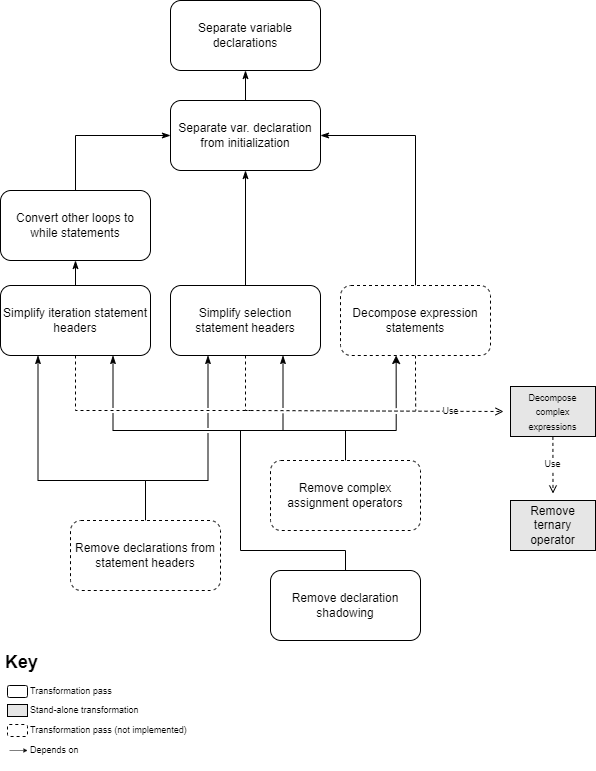
\includegraphics[width=\textwidth]{transformations.png}
    \caption{Dependency diagram of the envisioned transformations, their implementation status, and auxiliary transformations.}
    \label{fig:transform-diagram}
\end{figure}

Figure \ref{fig:transform-diagram} illustrates the dependencies between each transformation. Furthermore, because not all transformations were implemented, their implementation status is made explicit. Finally, we show where some auxiliary transformations are used.

After these transformations, we come to have a normalized program that is ready for further analyses and optimizations to be applied.

\section{Conclusion}

In this chapter we have discussed the factors that lead compiler developers to opt for more or less complex intermediate languages, outline the two main goals for our intermediate language - simplified but structured control flow, and explicit separation of expression value, control flow and side-effect evaluation - and their implications, and contribute a schedule of transformations that, when applied to a program, yield an equivalent program in a normalized subset of the source language.

\chapter{Case Study: Source-to-source function inlining and enabling effects of normalization}\label{chap:inlining}

\section{Inlining as a concept}

Function inlining is an optimization that substitutes a call to another procedure for the body of that very same procedure. For example, take the following code example, which uses a helper function to calculate the offset to take into a linear buffer corresponding to a matrix:

\begin{lstlisting}
size_t matrix_offset(size_t n_cols, size_t row, size_t col)
{
    return n_cols * row + col;
}

// size_t n_rows;
// size_t n_cols;

for (size_t i = 0; i < n_rows; i++)
{
    for (size_t j = 0; j < n_cols; j++)
    {
        size_t offset = matrix_offset(n_cols, i, j);
        // do something with the offset
    }
}
\end{lstlisting}

If targeting an imaginary stack machine, but one where local variables can be stored in unlimited virtual registers, a naive translation of this code would yield machine code like:

\begin{lstlisting}
procedure matrix_offset:
  pop r0 // n_cols
  pop r1 // row
  pop r2 // col
  pop r4 // return address
  
  r5 = r0 * r1 // temporary, row offset
  r6 = r5 + r2
  
  push r6
  jmp r4
end procedure

procedure main
  // r0 is n_rows
  // r1 is n_cols
  
  r2 = 0 // i
label loop_1
  jmp_gt_eq r2, r0, end_loop_1
  
  r3 = 0 // j
label loop_2
  jmp_gt_eq r3, r1, end_loop_2
  
  push offset_return
  push r3
  push r2
  push r1
  jmp matrix_offset
label offset_return:
  pop r4 // offset
  
  // ... do something with r4
  
  r3 = r3 + 1
  jmp loop2
label end_loop2

  r2 = r2 + 1
  jmp loop1
label end_loop1
end procedure
\end{lstlisting}

From this listing, one can see already one of the overheads associated with function calls. Depending on the calling convention, the system must perform extra copies of the arguments that are used to pass into the called procedure, either storing them in the stack (main memory) or in specific registers. Furthermore, if the architecture of the system does not allow an unlimited number of registers, it must save any other relevant values stored in the registers to memory, to prevent them being modified by the called procedure. Finally, the two procedures can be located in very disparate parts of memory, so performance may suffer because of decreased colocality on memory.

Let us now consider the same code processed by an inlining step, followed by some basic copy elision for clarity's sake, yielding the following code:

\begin{lstlisting}
procedure main
  // r0 is n_rows
  // r1 is n_cols
  
  r2 = 0 // i
label loop_1
  jmp_gt_eq r2, r0, end_loop_1
  
  r3 = 0 // j
label loop_2
  jmp_gt_eq r3, r1, end_loop_2
  
  r4 = r1 * r2 // temporary, row_offset = n_cols * i
  r5 = r4 + r3 // offset
  
  // ... do something with r5
  
  r3 = r3 + 1
  jmp loop2
label end_loop2

  r2 = r2 + 1
  jmp loop1
label end_loop1
end procedure
\end{lstlisting}

Several aspects here are improved. Firstly, there ceases to be a need for branching into remote code locations, which, coupled by the increased code locality, might decrease the CPU stalling associated to instruction cache misses and branch mispredictions. Secondly, access to the data memory is reduced. On our abstract machine stack access is completely eliminated, since the function parameters can be set by copying parameters to new registers (these copies were later elided for code clarity, but nevertheless access to them would be more performant than performing reads and writes to memory), but even in machines where the number of registers is limited, this inlining may be beneficial because of reduced stack spilling of registers during register allocation. Finally, having full access to the code of the called procedure could enable further optimizations. For example, now that a global analysis of the main function can see that the matrix offset computation is actually constituted by a loop-invariant row offset computation and a loop-variant addition, it could hoist the first part of the computation to the outer loop.

\section{Inlining in a source-to-source context}

Conceptually speaking, inlining should be a relatively simple operation. The compiler must take the text of the called function, replace the call with said text, adjust references to the arguments of the function to point to the parameters passed into the call, and store the resulting expression, if it gets used in the called context. Indeed, in the example presented in the previous section, that can be quite easily done. One must only assign to the lvalue of the call the expression contained in the return statement, and replace the arguments of the function declaration with those of the call:

\begin{lstlisting}
size_t matrix_offset(size_t n_cols, size_t row, size_t col)
{
    return n_cols * row + col;
}

// ... size_t n_cols, i, j;
size_t offset = matrix_offset(n_cols, row, col);
// becomes
size_t offset = n_cols * i + j;
\end{lstlisting}

However, in the general case, high-level languages such as C and C++ do not exhibit a strict separation between assignment expressions, side-effects and control flow, and syntax for statements and expressions is not perfectly composable, so there are many factors that will impede this straight-forward implementation of inlining. In the course of this section, we present several factors that impede this implementation, and how the normalization process described in Chapter \ref{chap:subset} or further transformations might enable implementing this transformation in an increased number of situations.

\subsection{References to caller lvalues and mutation of function parameters}

The first aspect that we must take into consideration is the fact that C and C++ function calls provide their parameters by value. This means that a function can modify the value of its parameters, without modifying said values on the caller's end.

The concrete implication this has for our inlining transformation is that we must copy all call arguments and reference those copies in the inlined function code, as opposed to directly referencing the parameter values. If there is a significant performance impact stemming from these copies, we could implement a copy elision step afterwards, to remove unneeded duplication.

\subsection{Calls contained in compound expressions and statement headers}

The second aspect we consider is that, in C and C++, function calls can be nested in contexts where the text of the function (which can be comprised of several statements, including declarations and control flow statements) cannot be inlined in a way that is syntactically valid, such as where the language only allows expressions to be placed, like in compound expressions and in selection or iteration statement headers.

However, calls as an expression statement, and assignment from the return value of a call to an lvalue, in the context of a scope, can always be inlined, by inlining the text of the called function and, if the return is not void, assigning the would-be returned expression to the left hand side of the original assignment.

Taking into this consideration, we can consider that the transformations detailed in Section \ref{sec:subset-expressions} enable us to perform inlining in more cases, by extracting expression evaluation from statement headers, and decomposing expressions into simpler expressions that will end up reduced to the trivially supported cases outlined above.

\subsection{Early return statements}

While C and C++ generally feature structured control flow, early return statements allow a function to break that structured flow and jump over executed code. When inlining functions that make use of that ability, the assumption that a return statement can simply be replaced with an assignment to a variable containing the result is no longer valid, an thus impede the straight-forward implementation of inling.

As mentioned in Section \ref{sec:subset-control-flow}, we do not think it wise to remove this facility in general, but, for the inlining of calls to functions that feature early returns, we devised a transformation that would make it so that only a single-return remains: an output variable is declared at the beginning of the function's scope, and a labeled return statement is introduced at the end of the function's text, returning said output variable. Then, all other return statements are replaced with a combination of assignments to the output variable, and unconditional jumps to the labeled return at the end of the function, as shown in Section \ref{sec:inlining-impl}.

\section{Implementation}\label{sec:inlining-impl}

Finally, having discussed these conditions and after applying transformations to normalize the program to our language subset, we are able to implement a transformation to inline function calls.

First, we must ensure two pre-conditions:

\begin{itemize}
    \item The call in question is either a top-level expression statement within a scope, or is the right side of a top-level assignment expression statement. This is ensured by the normalization process we applied beforehand.
    \item The inlined function does not access variables which the caller cannot access (e.g. the function and the caller are in different translation units and the function accesses global variables that use internal linkage, or a C++ class's member or friend function accesses private fields of the class and is called in an external context). We are not currently verifying this condition, as we do not think it necessary for a prototypical implementation, so the calls to be inlined must be chosen with care.
\end{itemize}

Then, to ensure that the function is able to be inlined, we apply two preliminary transformations to it: we transform the function, as described before, to ensure that only a single return statement is made, at the end of the function's text. Then, we process the variable names to ensure that there is no shadowing. This ensures that further transformations based on variable names do not need to handle possible variable shadowing.

Finally, we are able to perform the transformation, in source form, through the following steps:

\begin{enumerate}
    \item Replace the call or assignment in the caller with an empty scope.
    \item Insert variable declarations corresponding to the function's arguments, and assign the value of the call's arguments to those variables.
    \item Copy over the nodes corresponding to the function's body.
    \item If the function returns a value, and the caller assigned the value of the call to a variable, replace the return statement with an assignment, whose left hand side is the caller's result variable and the right hand side is the function's return expression.
    \item Rename any variable that needs it to ensure that the naming does not conflict with the caller's variables.
\end{enumerate}

To provide a concrete example, in the following code:

\begin{lstlisting}
int *get_elem(int *slice, size_t size, size_t offset)
{
    if (offset >= size)
    {
        return NULL;
    }

    return slice + offset;
}

// int *slice;
// size_t size;
// size_t i;

int *elem = get_elem(slice, size, i);
}
\end{lstlisting}

Firstly, the normalization occurs:

\begin{lstlisting}
int * get_elem(int *slice, size_t size, size_t offset) {
   int decomp_1;
   decomp_1 = offset >= size;
   if(decomp_1) {
      
      return ((void *) 0);
   }
   
   return slice + offset;
}

// int * slice;
// size_t size;
// size_t i;
int *elem;
elem = get_elem(slice, size, i);
\end{lstlisting}

Then, the function \verb|get_elem| is prepared to be inlined:

\begin{lstlisting}
int * get_elem(int *slice, size_t size, size_t offset) {
   int *__return_value;
   int decomp_1;
   decomp_1 = offset >= size;
   if(decomp_1) {
      __return_value = ((void *) 0);
      goto __return_label;
   }
   __return_value = slice + offset;
   goto __return_label;
   __return_label:
   
   return __return_value;
}
\end{lstlisting}

Note that the non-structured control flow is made explicit and only a single return statement remains. Finally, the inlining is able to be carried out:

\begin{lstlisting}
int * get_elem(int *slice, size_t size, size_t offset) { /* ... */ }

// int * slice;
// size_t size;
// size_t i;
int *elem;
{
    int * __inline_0_slice = slice;
    size_t __inline_0_size = size;
    size_t __inline_0_offset = i;
    int *__inline_0___return_value;
    int __inline_0_decomp_1;
    __inline_0_decomp_1 = __inline_0_offset >= __inline_0_size;
    if(__inline_0_decomp_1) {
       __inline_0___return_value = ((void *) 0);
       goto __return_label;
    }
    __inline_0___return_value = __inline_0_slice + __inline_0_offset;
    goto __return_label;
    __return_label:
    elem = __inline_0___return_value;
 }
\end{lstlisting}

This transformation was implemented in an Inliner class, available on the Clava standard library, through the methods \verb|inline($exprStmt)|, which inlines a single call, and \linebreak \verb|inlineFunctionTree($function)|, which recursively inlines all calls made in a function, as well as in the functions that are called.

\chapter{Experimental Evaluation}\label{chap:evaluation}

Having developed a set of transformations to normalize C and C++ programs to the theorized language subset, and having implemented an inlining optimization that takes advantage of the enabling effects of the normalization process, we devised three experiments to validate our approach:

\begin{enumerate}[label=\Alph*]
    \item Comparing a pre-existing inlining transformation's effectiveness with and without normalization, and comparing its effect to the new inlining transformation, which fully accounts for the normalization's effect.
    \item Determining the performance effects of the developed inlining optimization.
    \item Determining the enabling effects, if any, of the normalization transformations on the performance of a source-to-source automatic code parallelization tool.
\end{enumerate}

\section{Experiment A: Comparison of function inlining implementations with and without normalization}

Besides the inlining transformation that we implemented and described on Chapter \ref{chap:inlining}, the Clava standard library already possessed a previously implemented prototype of an inlining transformation, accessed through calling the \texttt{inline} method on a call node in the AST.

To compare both implementations, as well as the enabling effect of the normalization, a set of three synthetic benchmark programs were developed, featuring a variety of function calls in different contexts of the language:

\begin{itemize}
    \item A program generating 1,200,000 random two-dimensional observations and clustering them into 8 classes using a K-Means algorithm.
    \item A program multiplying two rank-35 square matrices and computing the trace of the resulting matrix.
    \item A program generating an array of 1,000,000,000 random natural numbers and performing a set of aggregations on them.
\end{itemize}

With these programs as our targets, we then proceded to run Clava to normalize and inline them as much as possible, under the following four configurations:

\begin{enumerate}
    \item Old: Using the previously implemented inlining transformation, try to inline all calls in the test programs.
    \item Normalize + Old: Normalize the test programs, then try to inline all calls with the previously implemented transformation.
    \item New: Using the newly implemented inlining transformation, try to inline all calls in the test programs.
    \item Normalize + New: Normalize the test programs, then try to inline all calls with the newly implemented transformation.
\end{enumerate}

As an evaluation metric, we chose to use the number and ratio of calls that were able to be inlined.

\begin{table}
\centering
\begin{tabular}{|c | c c c c |}
    \hline
    Scenario & \# Calls & \# No function body  & Calls Inlined & Inlining Failures \\
    \hline
    Old & 46 & 31 & 2 & 13 \\
    Normalize + Old & 50 & 31 & 6 & 13 \\
    New & 46 & 31 & 6 & 9 \\
    Normalize + New & 50 & 31 & 19 & 0 \\
    \hline
\end{tabular}
\caption{Effects of different inlining implementations with and without normalization.}
\label{tab:inlining-results}
\end{table}

Table \ref{tab:inlining-results} shows the results of the experiment. As evidenced on the first results column, we see that the normalization results on an increased number of calls being present. This is an effect of our normalization passes, namely passes to decompose expressions on the headers of iteration and selection statements, duplicating code to preserve the semantics of the normalized program. Furthermore, we see on the second column that there is a significant number of function calls that are not elegible to be inlined, owing to the body of the function not being present in the translation units that are being considered. In our case, these are calls to the C standard library, which is linked dynamically to the program.

The last two columns provide us with more interesting details.

First, we can observe the results of the program normalization. Compared with the scenarios where no normalization was made, the normalized programs are easier to inline (the old inliner goes from inlining ca. 13\% of elegible calls to inlining ca. 32\% of elegible calls, and the new inliner goes from inlining 40\% of elegible calls to inlining 100\% of elegible calls). The reason for this improvement is that, by decomposing complex expressions and by removing those expressions from the headers of control statements and other calls, we get a greater number of isolated calls and simple assignments from the value of a call to a variable, which are feasible cases for source-to-source inlining.

Secondly, we can perform a direct comparison of the two inlining implementations. From inspection of the Clava source-code, we see that to implement the inlining transformation in a less abstract language, such as Java for the case of Clava, cases where implementation can apply must be explicitly enumerated, whereas when implementing the transformation on the Javascript environment, we can rely on structural analysis and exception handling to make the transformation more general, while catching errors that pop up as exceptions. This is reflected on the comparative results of both approaches. The previously implemented inliner, which featured the exhaustive approach in Java, fails to inline calls in several occasions due to not recognizing the nodes contained within the body of the function, whereas the Javascript-based transformation need not concern itself with that filtering, leading to a ca. 27 pp. increase of successful transformations with no normalization, and, leveraging the simplification of the language afforded by the normalization process, can reach a 100\% successful inlining rate, a 68 pp. increase over the \texttt{Normalize + Old} scenario.

To validate these results, we compiled and ran the original and transformed programs, and verified that the expected output remained the same. In the case of the first scenario, additional care had to be taken to extract a useful copy of the transformed code, since one of the inlining applications produced a structuraly unsound program, therefore we saved and restored the AST before and after each inlining we tried.

There are, naturally, some factors that might affect the validity of our results:

\begin{itemize}
    \item The number and nature of the programs that we tested do not constitute an exhaustive sample of all the language constructs that a C program might contain, much less all of the constructs contained in a C++ program. There is a strong possibility that there are language features that are not accounted for and might necessitate changes and/or additions to the normalized subset or the normalization process. Nevertheless, we believe that this approach is extensible enough to bound the complexity of the resulting subset, at least for C programs and reasonably simple C++ programs used in scientific computing.
    \item The two approaches to inlining may not be strictly comparable in terms of complexity, since the older implementation takes care of some other concerns such as function body caching that the new implementation does not. However, an analysis of the implementation led us to believe that the monolithic nature of the old implementation, especially by having to deal with all the complexities of the source language, as opposed to the subset we had previously defined, played a part in its reduced flexibility.
\end{itemize}

\section{Experiment B: Performance Effects of Inlining}

To evaluate the performance effects of inlining, we took the same programs and benchmarked their runtime performance, with and without inlining, using a variety of compilers and different optimization settings. Specifically, we compiled the original and transformed programs using the GCC, clang, and CompCert toolchains, both under the \texttt{O0} (no optimizations enabled) and the \texttt{O2} (standard optimizations) optimization levels, performing, for each combination of program, compiler, presence of inlining transformation and optimization level, and measuring the average runtime duration. Inlining was performed for the entire program, by traversing the program's call graph in a depth-first fashion and inlining all calls.

We expected the following results:

\begin{itemize}
    \item Under the \texttt{O0} optimization level, we expected that, besides generally slower runtime performance, we would see a clear performance impact of the inlining transformation, varying in its sign and magnitude depending on the trade-off between the number of times a certain call is performed, and the code bloat resulting from the duplicated function bodies. Specifically, we theorized that inlining small functions that are called often would result in performance gains, and that inlining bigger functions with less frequent calls would have smaller gains or even negative performance effects.
    \item Under the \texttt{O2} optimization level, we expected that there would be little performance effect, as the compilers under test already should perform several code optimization transformations, including inlining, and so the source-code level transformation would have less of an effect.
\end{itemize}

\begin{figure}
    \centering
    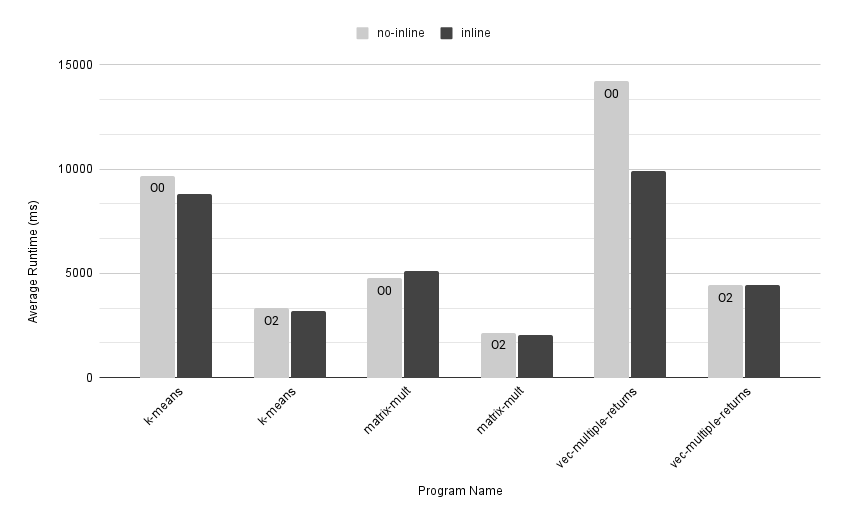
\includegraphics[width=\textwidth]{figures/benchmark-chart.png}
    \caption{Microbenchmark performance, inlining vs no inlining. Segmented by program, optimization level.}
    \label{fig:expb-chart}
\end{figure}

Figure \ref{fig:expb-chart} shows a high-level visualization of the results of this experiment. For each program, two sets of columns show the average runtime in several configurations. One set presents the results with no compiler optimizations (\texttt{O0}) and the other presents the results with optimizations enabled (\texttt{O2}). The columns in light grey show the average runtime of the original program for that configuration, and the columns in dark grey show the average runtime of the program after the source-level inlining was applied.

In aggregate, the results obtained fell within the expectations we had set before. The \texttt{k-means} and \texttt{matrix-mult} programs, that featured larger functions and less iterations comparatively to the number of calls, had less expressive and mixed performance impacts on the runtime performance of the program when transformed. Specifically, on the \texttt{O0} configuration, K-Means compute performance was ca. 9\% faster, but Matrix Multiplication was ca. 7\% slower. On the other had, the \texttt{vec-multiple-returns} program, which featured a tight-loop more easily dominated by a call to a small function, experienced a ca. 30\% reduction in average runtime. Under the \texttt{O2} configuration, the performance effects were generally less expressive, as expected, but, surprisingly, we saw an inversion on the magnitudes of the performance effects when comparing k-means and matrix multiplication with the array slice aggregation program. While the performance effect on \texttt{vec-multiple-returns} dropped to ca. -0.34\%, source-level inlining decreased the average runtime of \texttt{k-means} and \texttt{matrix-mult} by ca. 4.5\% and 5.2\%, respectively. A possible explanation is that the underlying compilers might not have inlined certain calls, without the source-level inlining, and the inlined function would enable more optimizations to be performed at the global analysis level.

\begin{table}[]
\centering
\begin{tabular}{|c|c|c|ccc|}
\hline
\multirow{2}{*}{Compiler} & \multirow{2}{*}{Opt. Level} & \multirow{2}{*}{Inlining} & \multicolumn{3}{c|}{Program} \\
\cline{4-6} 
 & & & vec-multiple-returns & matrix-mult & k-means \\
\hline
\multirow{4}{*}{CompCert} & \multirow{2}{*}{O0} & Yes & 4462.37 & 2864.06 & 3392.99 \\
 & & No & 4454.64 & 2792.85 & 4630.94 \\
 & \multirow{2}{*}{O2} & Yes & 4443.17 & 2694.85 & 4379.61 \\
 & & No & 4445.98 & 2796.52 & 4830.31 \\
\hline
\multirow{4}{*}{Clang} & \multirow{2}{*}{O0} & Yes & 6723.64 & 6376.61 & 11379.62 \\
 & & No & 19771.91 & 5714.09 & 11717.30 \\
 & \multirow{2}{*}{O2} & Yes & 4418.02 & 1619.00 & 1972.17 \\
 & & No & 4420.98 & 1889.16 & 1978.27 \\
\hline
\multirow{4}{*}{GCC} & \multirow{2}{*}{O0} & Yes & 18486.90 & 6059.89 & 11662.09 \\
 & & No & 18456.40 & 5784.92 & 12703.43 \\
 & \multirow{2}{*}{O2} & Yes & 4451.80 & 1840.78 & 3182.59 \\
 & & No & 4401.42 & 1806.91 & 3173.13 \\
\hline
\end{tabular}
\caption{Runtime performance (ms) for each program, segmented by compiler, optimization level, source-level inlining.}
\label{tab:expb-pivot}
\end{table}

Zooming in from the aggregate results to the results separated by compiler, we come upon other interesting results. Table \ref{tab:expb-pivot} shows the runtime performance numbers, segmented by compiler, optimization level, and whether source-level inlining was applied. There, we can see that the results actually follow two modes regarding the behavior presented by different compilers. Clang and GCC, which are older but have had more optimization work put it, present a stark difference between the code that is generated with and without optimization. On the other hand, CompCert seems to generate comparatively faster code without optimizing, but does not present large gains in performance when code optimization is enabled. Comparing both sets, we see that the optimized code from GCC and Clang seems to be faster than optimized code from CompCert. Nevertheless, source-level inlining seems to be worthwhile in general, especially when considering that the transformations that we developed were prototypical and limited in nature, so further work may result in even greater performance effects. In some cases, there is a sizable performance benefit of applying it, such as on array slice aggregation with O0 and Clang, and on k-means with CompCert, in which it performs faster than even the optimized code, supporting our hypothesis that source-to-source transformation work will be especially impactful on less developed compilers.

To validate our results, we measured, for each configuration, 8 runs of the benchmark. Besides recording the average runtime duration, we recorded the standard deviation of our observations. For \texttt{vec-multiple-returns} and \texttt{k-means}, the average standard deviation of our observations was well under 1\% of the measured average runtime duration. For \texttt{matrix-mult}, the measurement standard deviations were somewhat higher, but still within 10\% of the magnitude of the observations in all cases.

Of course, some factors do limit our analysis and confidence in these results:

\begin{itemize}
    \item The programs that we tested only represent a subset of the types of computation performed in C and C++, and thus the results might not be representative of the effect of the transformation on the overall corpus of existing C and C++ code. A larger set of codes might be tested to further validate the results.
    \item Only one hardware target was used in the test and, by extension, only one set of platforms and computation models. As an extension, it might prove useful to test this optimization on different platforms, different hardware targets (featuring different single-clock speeds, cache sizes, etc.) and different computation models (GPU, FPGAs with HLS, etc.).
    \item We only developed and tested one optimizing transformation. Other transformations might be more or less worthwhile to be executed at different levels of abstraction, and so we may not draw overly general conclusions about the potential use of the source-to-source compilation approach to optimization.
\end{itemize}

Nevertheless, we can conclude that there are some measurable effects of performing inlining on the source-code level on the performance of certain C and C++ programs, under different compilers.

\section{Experiment C: Enabling Effects of Normalization on Automatic Parallelizer}

The last experiment we performed was running a well-known benchmark through an existing source to source optimization tool to validate the effect of our normalization code. To do so, we selected the following benchmark and tool:

\begin{itemize}
    \item As the benchmark, we selected the NAS Parallel Benchmarks. These benchmarks, originally produced by NASA, aim to test the performance of parallel computing systems, which paired well with the tool we chose. Furthermore, an implementation of these benchmarks was already packaged in a compatible way with the LARA Framework's benchmark facility.
    \item As the tool to test, we chose Autopar-Clava\cite{Arabnejad2018}, an automatic parallelization transformation for Clava. This tool  analyses a program's loops, its inductive variables, and its memory access patterns \cite{Arabnejad2020} to insert OpenMP directives in the code, yielding a parallelized version of it. We chose it for our evaluation due to its presence in the Clava standard library, as well as previous expertise in the lab developing and using it. Furthermore, Autopar-Clava was described by its authors as using Clava's built-in inlining facility, so we hoped to be able to compare this implementation to our own newly-implemented inlining facility.
\end{itemize}

We aimed this experiment to explore the enabling effects of the newly developed normalization and inlining transformations on the effect of further optimizations. Thus, from the NAS benchmark suite, we picked a variety of tests, in several classes of magnitude. We chose the tests in a way that ensured a variety of source-code constructs was represented, and chose the magnitudes that would be big enough to ensure confidence in the results, yet not too large, in the interest of time. Specifically, we picked benchmarks for a Block Tri-diagonal matrix equation solver (BT), a Conjugate Gradient computation kernel for linear differential equation solving (GG), a discrete 3D fast Fourier Transform computation kernel (FT), a Lower-Upper matrix solver using the Gauss-Seidel method (LU), a differential equation solver kernel using the Multi-grid method (MG), and a Scalar pentadiagonal matrix solver (SP), using the magnitude classes W, A, and B, which range in runtime duration from ca. 0.5 seconds to ca. 8 minutes.

Afterwards, we laid out four scenarios:

\begin{enumerate}
    \item Baseline: benchmark the selected benchmark instances, without modification.
    \item Autopar: parallelize the selected benchmark instances using Autopar-Clava, with no preceding transformations, and benchmark the transformed programs.
    \item Normalize: normalize the selected benchmark instances to our predefined language subset, parallelize them, and benchmark the tranformed programs.
    \item Inline: modify Autopar-Clava to disable the built-in inlining transformation; normalize the selected benchmark instances to our predefined language subset, perform automated inlining with our newly developed inlining transformation, parallelize them, and benchmark the transformed programs (this scenario remained untested).
\end{enumerate}

As an evaluation metric, we again chose the runtime duration of the benchmarks, seeking to minimize it. Our expectation was that Autopar-processed code would perform better than the baseline on our multi-core workstation, with the exception of the FT benchmark, which was expected to slow down, as per the results previously obtained in \cite{Arabnejad2020}.

% Please add the following required packages to your document preamble:
% \usepackage{multirow}
\begin{table}[]
\centering
\begin{tabular}{|c|c|ccc|}
\hline
\multirow{2}{*}{Program} & \multirow{2}{*}{\begin{tabular}[c]{@{}c@{}}Magnitude\\ Class\end{tabular}} & \multicolumn{3}{c|}{Scenario}    \\ \cline{3-5} 
                         &                                                                            & Baseline & Autopar   & Normalize \\ \hline
\multirow{3}{*}{BT}      & W                                                                          & 5.32     & 22.87     & 5.41      \\
                         & A                                                                          & 113.46   & 59,979.11 & 118.31    \\
                         & B                                                                          & 468.25   & -         & 517.56    \\ \hline
\multirow{3}{*}{CG}      & W                                                                          & 0.57     & 0.05      & 0.59      \\
                         & A                                                                          & 2.00     & 0.11      & 2.04      \\
                         & B                                                                          & 90.21    & 7.07      & 95.97     \\ \hline
\multirow{3}{*}{FT}      & W                                                                          & 0.44     & 11.93     & 0.46      \\
                         & A                                                                          & 7.93     & 253.65    & 8.13      \\
                         & B                                                                          & 95.16    & 5,771.09  & 98.83     \\ \hline
\multirow{3}{*}{LU}      & W                                                                          & 16.46    & 61.10     & 18.31     \\
                         & A                                                                          & 112.25   & 947.73    & 116.44    \\
                         & B                                                                          & 467.46   & 6,247.38  & 481.04    \\ \hline
\multirow{3}{*}{MG}      & W                                                                          & 0.58     & 0.08      & 0.64      \\
                         & A                                                                          & 4.62     & 0.60      & 5.04      \\
                         & B                                                                          & 20.98    & 1.85      & 22.94     \\ \hline
\multirow{3}{*}{SP}      & W                                                                          & 18.40    & 23.71     & 19.43     \\
                         & A                                                                          & 104.44   & 164.17    & 110.02    \\
                         & B                                                                          & 437.79   & 706.49    & 458.73    \\ \hline
\end{tabular}
\caption{Runtime duration of benchmarks (s), segmented by scenario, program, magnitude class.}
\label{tab:expc-results}
\end{table}

Table \ref{tab:expc-results} shows the resulting runtime duration for each of our scenarios. Compared to the baseline, the Autopar scenario showed definite effects on the runtime performance of different benchmarks. In the case of the CG and MG program, we were able to obtain concrete speedups, on the order of 7.25x to 18.18x. FT also performed as seen in \cite{Arabnejad2020}, being several tens of times slower than the baseline result. However, we could not reproduce the results previously seen for the BT, LU and SP cases. In the case of LU, slight slowdowns occured. In the case of LU and BT, though, the performance degradation seemed to scale with the benchmark magnitude super-linearly, leading to not being able to obtain any results for BT at magnitude class B. We suspected that the two-chiplet design of our workstation's CPU could be to blame for the slowdown, owing to slower communication between cores, but we were also unable to reproduce these results using codes from the original publication and on another workstation, which did not share the same hardware peculiarities. Another hypothesis for the slowdown was that the loops that were parallelized did not perform enough work on their own, so the overhead of parallelizing them resulted in performance degradation.

Compared to the previous two scenarios, the Normalize scenario evidenced a surprising result. Autopar-Clava was not able to parallelize any loops, and thus the runtime performance was roughly similar to the baseline scenario, as opposed to being similar to the Autopar scenario. Analyzing the output logs, we realized that Autopar relied on analyzing \texttt{for} statements to identify possible parallelization opportunities. Since our normalization transformation removed \texttt{for} statements from the language subset, the parallelizer was not able to perform its job. In the absence of more time for reworking the normalization transformations to account for this use, we carried out with analyzing the results of this experiment and drawing conclusions, having cancelled testing for scenario Inline, since the same lack of results was certain.

This experiment showed us that there is still room for reconsideration of the subset that we defined. For statements are an important expressive construct for use in writing a program but, guided by the fact that compilers are able to identify loop structures, their invariants and induction variables, we considered on a theoretical sense that they would not be necessary on our language subset. However, even if not strictly necessary, the construct is used for automated tools and analyses in a source-to-source context, and thus removing it may not be the best decision. To reintroduce the construct into the subset, we might consider the following two routes:

\begin{itemize}
    \item Only transforming for loops into while loops conditionally, based on the characteristics of the statements in the header. For example, we could keep simple loops, such as a canonical loop comparing against a constant or variable, while processing loops that compare against the return value of a call. \textit{In extremis}, we could rely on user input of some sort to mark instances to be kept.
    \item We can keep our transformation to a while loop, and then follow it with passes for loop canonicalization, such as loop invariant code motion, induction variable analysis and so on, reconstituting a normalized version of the for loop afterwards. This approach is certainly more complex, but might work better in the general case.
\end{itemize}

\section{Summary}

In this chapter, we presented three experiments to try and understand how source-code normalization affects the possibility and ease of implementing program optimizations on the source-code level. The first experiment showed that after normalizing the code, two independent implementations of a function inlining transformation were able to inline calls in more situations that they were able to before. The second experiment validated our case study in implementing a performance optimization in a source-to-source context, since performance effects of the transformation were evident, especially on less optimizing compiler choices and configurations. The third experiment had negative results. Besides having had trouble reproducing a baseline that was in line with previous works on the tool we chose, our normalization process removed primitives on which the tool relied and greatly diminished its effect. While not invalidating our approach, it gave us a perspective on how our work can be improved upon.

\chapter{Conclusions}\label{chap:conclusions}

When considering conclusions, we think that our work can be considered in several different facets. We first considered our literature review work, followed by work of theorizing a language subset that would meet our criteria. Then we considered the implementation of our normalization work and its results, and finally considered our case study in organization.

Regarding our survey of relevant literature, we consider that we were largely successful in identifying the breadth of approaches that are currently being investigated or implemented to tame the complexity of optimization work, even if not at great depth. We think that our survey of approaches tailored towards more heterogeneous systems could have had more depth, but then again the lack of surveys in this area, coupled with more practical goals, did not allow further exploration. Nevertheless, we identified many limitations that guided the research questions and ultimately our proposed solution and contributions.

We think that our main contribution was establishing a suitable theoretical framework for building a subtractive subset of C and C++, especially considering the sheer breadth and depth of constructs of these high-level languages. We think that the principles that we identified will be foundational and useful when applying this exercise to other languages and scenarios and, even if the subset that we derived was by no means exhaustive or perfectly adequate, it will surely serve as a good first draft to keep iterating on a better C or C++ subset that could be targeted by source-to-source compiler users to perform analyses and transformations. Generally speaking, we think we were successful in meeting our objectives along this facet.

Our case study on function inlining also produced successful results. Our normalization pass was able to enhance the action of pre-existing and newly implemented inlining transformations and we observed promising performance results when benchmarking the effect of inlining on the runtime duration of sample programs.

Our experiment to evaluate our normalization pass's interaction with other optimizations was not so successful. Besides having trouble reproducing work by earlier authors, we neutered the performance effect of their contributions with our transformation. This is a disappointing result, but allowed us to understand some limitations of the subset we have currently defined, and will surely guide a future version of the subset that will be able to avoid those problems.

\section{Contributions}

On a more exhaustive note, we think that we were able to present several contributions along diffent axes:

\begin{itemize}
    \item Producing a high-level survey of different approaches for taming the complexity of high-level languages, with the aim of making them more amenable for analyses and transformations, and heterogeneous compilation targets, such as mid-level IRs, multi-level IRs, declarative transformations, and discussion of their limitations and tradeoffs, \textit{viz.} in comparison with source-to-source compilation approaches.
    \item Adopting a structure for source-code transformations in Lara and Clava, especially for the use case of automated transformation, as was the case of the Pass abstraction, common in other compilers but previously unused in our immediate context.
    \item Adopting a set of principles that could guide the production of an analysis-friendly subset of an imperative programming language.
    \item Implementing a suite of automated transformations that could transform a large subset of C programs and simpler C++ programs into a normalized subset of the language that was more amenable for source code transformation.
    \item Discussing the challenges present in designing a code inlining transformation in a source-to-source compilation context.
    \item Producing a simple, yet effective code inlining transformation that leverages the aforementioned normalization pass.
    \item Practical evaluation experiments and results that highlight the advantages and deffects of our implementation, as well as some tradeoffs of our approach.
\end{itemize}

\section{Future Work}

There are some limitations in our work that could be addressed in the future:

\begin{itemize}
    \item Having co-developed our theoretical framework for normalization and our implementation of such transformation, there are several mismatches between what the framework demands, the specification we derived, and the implementation we built, that produce less than ideal results in terms of readability, program correctness and expressiveness. Further work is needed to bring these factors into alignment. Specifically, we would like to see further work on loop constructs and loop normalization, a more balanced approach to implementing complex expression decomposition (our implementation was particularly overzealous), and deriving more elements of the subset covering aspects that were not considered in the interest of keeping a narrow scope, such as C++ specific constructs such as classes, visibility and templates, atomics, or static and thread local storage.
    \item Further work is needed to validate the compatibility of our normalization with other programs, other compiler toolchains, other computing platforms and models, and so on. The same can be said for our inlining implementation.
    \item The Pass abstraction that was introduced to the LARA framework was a step forward in organizing successive code transformations in a declarative way. However, further work is still needed, especially investigating the possibility of doing automatic dependency resolution between passes, as well as checking desirable properties of transformation passes, such as idempotency.
    \item On Clava, further work can be done to integrate other alternative approaches and representation besides high-level languages. With the emergence of MLIR as a standard for interoperable IRs, it could be interesting to try to integrate the two approaches, especially as an alternative to the C++ and visitor-based extension patterns of that technology.
    \item The implementation itself needs further maintenance and improvement work. We would like to see work on other ways of improving ergonomics of Clava users, including access to more modern aspects of the Javascript environment, such as ES Modules and gradual typing with Typescript, DSLs for testing, integration with common Integrated Development Environments (IDEs) and protocols such as VSCode, IntelliJ and the Language Server Protocol, as well as an easier building and installation story. 
\end{itemize}

We again express our hope that this work can be a foundation for another avenue of exploration within the compiler research world, and that other developers will be excited to work on successors to, and competitors of, this project. Compiler research deserves to be a topic that is approachable by all kinds of engineers, students and scientists, and we believe that transitioning to models that allow both high-level work and focused work on different layers of abstraction to be easier to work with is of foremost importance.

%% comment next 2 commands if numbered appendices are not used
\appendix
\chapter{Validation and Benchmarking: Experimental Setup and Codes} \label{ap:validation}

To perform the validation of our technique, tests were run on a workstation with the following configuration:

\begin{itemize}
    \item CPU - AMD Ryzen Threadripper 3960X - 24 Cores with 2-way SMT, clocked at 2.2GHz, boosting to 4.5GHz
    \item RAM - 2x16 GiB at 3200 MT/s, in dual channel
    \item OS - Ubuntu 18.04.6 LTS
    \item Java - Azul Systems Zulu OpenJDK 11.0.5
    \item Compilers - clang v6.0.0 (experiment B), CompCert v3.10 (Coq platform v2022.04.1) (experiment B), gcc v7.5.0 (experiments B and C)
    \item Clava - built from source, commit 275e87b
    \item LARA Framework - built from source, commit 81bf5b62
    \item SPeCS Java Libraries - built from source, commit fa827db5
\end{itemize}

To build Clava from source, the repositories for Clava, the \href{https://github.com/specs-feup/lara-framework/tree/81bf5b624b0aa37ddd0bebda2b24e2a126f12609}{LARA Framework} and the \href{https://github.com/specs-feup/specs-java-libs/tree/fa827db586d7b2cbf94fff98873ee339f04cb694}{SPeCS Java Libraries} were cloned and imported into the Eclipse IDE, according to the instructions in the \href{https://github.com/specs-feup/specs-java-libs/blob/fa827db586d7b2cbf94fff98873ee339f04cb694/README.md}{SPeCS Java Libraries README file}, and the build target ClavaWeaver -> Java Application -> ClavaWeaverLauncher -> ClavaWeaverGUI was used to run the Clava toolchain.

\section{Experiment A}

\subsection{C Source Codes}

\subsubsection{K-Means}

Randomly distributes points around a set of pre-defined seed coordinates, and runs k-means to find clusters of points.

\begin{lstlisting}[caption=k\_means.c]
#include <stdio.h>
#include <stdlib.h>
#include <time.h>

float square_distance(float x1, float y1, float x2, float y2)
{
    float x_diff = (x1 - x2) * (x1 - x2);
    float y_diff = (y1 - y2) * (y1 - y2);
    float result = x_diff + y_diff;
    return result;
}

void calculate_centroid_means(size_t n_clusters, size_t gen_factor, float *centroid_xs, float *centroid_ys, size_t *centroid_counts, float *xs, float *ys, size_t *classes)
{
    // reset centroid means
    for (size_t k = 0; k < n_clusters; k++)
    {
        centroid_xs[k] = 0.0;
        centroid_ys[k] = 0.0;
        centroid_counts[k] = 0;
    }

    // update centroid means
    for (size_t i = 0; i < n_clusters * gen_factor; i++)
    {
        float x = xs[i];
        float y = ys[i];
        size_t k = classes[i];

        centroid_counts[k]++;
        centroid_xs[k] += (x - centroid_xs[k]) / centroid_counts[k];
        centroid_ys[k] += (y - centroid_ys[k]) / centroid_counts[k];
    }
}

int main()
{
    size_t n_clusters = 8;
    float cluster_seed_xs[8];
    cluster_seed_xs[0] = 3.0;
    cluster_seed_xs[1] = -2.1;
    cluster_seed_xs[2] = 12.8;
    cluster_seed_xs[3] = 0.3;
    cluster_seed_xs[4] = -7.5;
    cluster_seed_xs[5] = 16.2;
    cluster_seed_xs[6] = -13.1;
    cluster_seed_xs[7] = -0.7;
    float cluster_seed_ys[8];
    cluster_seed_ys[0] = 3.0;
    cluster_seed_ys[1] = 2.1;
    cluster_seed_ys[2] = -12.8;
    cluster_seed_ys[3] = -0.3;
    cluster_seed_ys[4] = 7.5;
    cluster_seed_ys[5] = 16.2;
    cluster_seed_ys[6] = -13.1;
    cluster_seed_ys[7] = -0.7;

    size_t allowed_switches = 2;
    size_t gen_factor = 150000;
    int dist_factor = 300;

    srand(42);

    float *xs = calloc(n_clusters * gen_factor, sizeof(float));
    float *ys = calloc(n_clusters * gen_factor, sizeof(float));
    size_t *classes = calloc(n_clusters * gen_factor, sizeof(size_t));

    // randomly distribute points around seed clusters
    for (size_t k = 0; k < n_clusters; k++)
    {
        size_t base = k * gen_factor;
        float cluster_x = cluster_seed_xs[k];
        float cluster_y = cluster_seed_ys[k];
        for (size_t offset = 0; offset < gen_factor; offset++)
        {
            size_t ix = base + offset;
            float x_delta = (rand() % (dist_factor * 2) - dist_factor) / (float)100;
            xs[ix] = cluster_x + x_delta;
            float y_delta = (rand() % (dist_factor * 2) - dist_factor) / (float)100;
            ys[ix] = cluster_y + y_delta;
            classes[ix] = rand() % n_clusters;
        }
    }

    // randomly distribute classes
    for (size_t i = 0; i < n_clusters * gen_factor; i++)
    {
        int class = rand() % n_clusters;
        classes[i] = class;
    }

    float centroid_xs[8];
    float centroid_ys[8];
    size_t centroid_counts[8];

    size_t switched_observations = 0;
    int iterations = 0;

    clock_t start, end;
    start = clock();
    do
    {
        switched_observations = 0;
        iterations++;
        calculate_centroid_means(n_clusters, gen_factor, centroid_xs, centroid_ys, centroid_counts, xs, ys, classes);
        for (size_t i = 0; i < n_clusters * gen_factor; i++)
        {
            float x = xs[i];
            float y = ys[i];
            size_t class = classes[i];

            for (size_t k = 0; k < n_clusters; k++)
            {
                float centroid_x = centroid_xs[k];
                float centroid_y = centroid_ys[k];
                float centroid_distance = square_distance(x, y, centroid_x, centroid_y);

                float class_x = centroid_xs[class];
                float class_y = centroid_ys[class];
                float class_distance = square_distance(x, y, class_x, class_y);

                if (centroid_distance < class_distance)
                {
                    class = k;
                }

                if (class != classes[i])
                {
                    classes[i] = class;
                    switched_observations++;
                }
            }
        }
    } while (switched_observations > allowed_switches);
    end = clock();
    fprintf(stderr, "%d\n", iterations);
    printf("%f\n", (end - start) / (double)(CLOCKS_PER_SEC / 1000));
}
\end{lstlisting}

\subsubsection{Matrix Multiplication and Trace}

Pre-populates two square matrices of similar rank, multiplies them, and gives the trace of the resulting matrix.

\begin{lstlisting}[caption=matrix\_mult.c]
#include <stdio.h>
#include <stdlib.h>
#include <time.h>
#include <stdbool.h>

typedef struct matrix
{
    size_t side;
    double **rows;
} matrix;

matrix *matrix_new(size_t sqrt_n)
{
    size_t side = sqrt_n * sqrt_n;
    double **rows = calloc(side, sizeof(double *));

    for (size_t row = 0; row < side; row++)
    {
        double *r = calloc(side, sizeof(double));
        rows[row] = r;
    }

    matrix *out = (matrix *)malloc(sizeof(matrix));
    out->side = side;
    out->rows = rows;

    return out;
}

void matrix_destroy(matrix *m)
{
    double **rows = m->rows;

    for (size_t row = 0; row < m->side; row++)
    {
        free(rows[row]);
    }

    free(rows);
    free(m);
}

double matrix_mult_coord(matrix *a, matrix *b, size_t i, size_t j)
{
    double acc = 0.0;

    for (size_t k = 0; k < a->side; k++)
    {
        acc += a->rows[i][k] * b->rows[k][j];
    }

    return acc;
}

void matrix_mult(matrix *a, matrix *b, matrix *out)
{
    size_t side = a->side;

    for (size_t i = 0; i < side; i++)
    {
        for (size_t j = 0; j < side; j++)
        {
            out->rows[i][j] = matrix_mult_coord(a, b, i, j);
        }
    }
}

void matrix_fill_rand(matrix *m)
{
    for (size_t i = 0; i < m->side; i++)
    {
        for (size_t j = 0; j < m->side; j++)
        {
            m->rows[i][j] = ((double)rand()) / 100.0;
        }
    }
}

double matrix_trace(matrix *m)
{
    double trace = 0.0;

    for (size_t i = 0; i < m->side; i++)
    {
        trace += m->rows[i][i];
    }

    return trace;
}

int main(void)
{
    srand(42);

    matrix *m1 = matrix_new(35);
    matrix *m2 = matrix_new(35);
    matrix *out = matrix_new(35);

    matrix_fill_rand(m1);
    matrix_fill_rand(m2);

    clock_t start = clock();
    matrix_mult(m1, m2, out);
    clock_t end = clock();
    printf("%f\n", (end - start) / (double)(CLOCKS_PER_SEC / 1000));
    double trace = matrix_trace(out);
    fprintf(stderr, "%f\n", trace);

    return EXIT_SUCCESS;
}
\end{lstlisting}

\subsection{Array Slice Aggregations}

Pre-populates a fixed array with random non-negative integers, and aggregates them.

\begin{lstlisting}[caption=vec\_multiple\_returns.c]
#include <stdio.h>
#include <stdlib.h>
#include <time.h>

int *slice_new(size_t size)
{
    return (int *)calloc(size, sizeof(int));
}

void slice_rand_fill(int *slice, size_t size)
{
    for (size_t i = 0; i < size; i++)
    {
        slice[i] = rand();
    }
}

int *slice_ref(int *slice, size_t size, size_t offset)
{
    if (offset >= size)
    {
        return NULL;
    }
    return slice + offset;
}

size_t slice_size(int *slice, size_t size)
{
    return size;
}

int main()
{
    srand(42);

    size_t size = 1000000000;
    int *slice = slice_new(size);
    slice_rand_fill(slice, size);

    unsigned int acc = 0;

    clock_t start = clock();
    for (size_t i = 0; i < slice_size(slice, size); i++)
    {
        int *elem;
        elem = slice_ref(slice, size, i);
        acc += (unsigned int)*elem;
        acc *= (unsigned int)*elem;
        acc += (unsigned int)*elem;
        acc *= (unsigned int)*elem;
        acc *= acc;
        acc += (unsigned int)*elem;
        acc *= (unsigned int)*elem;
        acc += (unsigned int)*elem;
        acc *= (unsigned int)*elem;
    }
    clock_t end = clock();
    fprintf(stderr, "%u\n", acc);

    printf("%f\n", (end - start) / (double)(CLOCKS_PER_SEC / 1000));
    return EXIT_SUCCESS;
}
\end{lstlisting}

\subsection{Clava Scripts}

These Clava scripts try to inline all possible calls in a given set of source-files, determined by the Clava config file, and report statistics about the inlinings.

\begin{lstlisting}[language=js,caption=Clava built-in inlining with no normalization]
laraImport("clava.code.Inliner");
laraImport("weaver.Query");

let calls_total = 0;
let calls_no_definition = 0;
let calls_inlined = 0;
let calls_inlining_fails = 0;

const inliner = new Inliner();

for (const call of Query.search("call")) {
  calls_total += 1;
  if (!call.function.isImplementation) {
    calls_no_definition += 1;
    continue;
  }
  try {
    println(
      `Trying to inline call '${call.code}' at location ${call.location}`
    );
    call.inline();
    println("Inlined successfully\n");
    calls_inlined += 1;
  } catch (e) {
    println(`Inlining failed: ${e.message}\n`);
    calls_inlining_fails += 1;
  }
}

println("Results:");
println(
  JSON.stringify(
    { calls_total, calls_no_definition, calls_inlined, calls_inlining_fails },
    undefined,
    2
  )
);
\end{lstlisting}

\begin{lstlisting}[language=js,caption=Clava built-in inlining with normalization]
laraImport("clava.code.Inliner");
laraImport("weaver.Query");
laraImport("clava.opt.NormalizeToSubset");
laraImport("clava.opt.PrepareForInlining");

let calls_total = 0;
let calls_no_definition = 0;
let calls_inlined = 0;
let calls_inlining_fails = 0;

NormalizeToSubset();

for (const call of Query.search("call")) {
  calls_total += 1;
  if (!call.function.isImplementation) {
    calls_no_definition += 1;
    continue;
  }
  try {
    println(
      `Trying to inline call '${call.code}' at location ${call.location}`
    );
    PrepareForInlining(call.function);
    call.inline();
    println("Inlined successfully\n");
    calls_inlined += 1;
  } catch (e) {
    println(`Inlining failed: ${e.message}\n`);
    calls_inlining_fails += 1;
  }
}

println("Results:");
println(
  JSON.stringify(
    { calls_total, calls_no_definition, calls_inlined, calls_inlining_fails },
    undefined,
    2
  )
);
\end{lstlisting}

\begin{lstlisting}[language=js,caption=Newly developed inlining with no normalization]
laraImport("clava.code.Inliner");
laraImport("weaver.Query");

let calls_total = 0;
let calls_no_definition = 0;
let calls_inlined = 0;
let calls_inlining_fails = 0;

const inliner = new Inliner();

for (const call of Query.search("call")) {
  calls_total += 1;
  if (!call.function.isImplementation) {
    calls_no_definition += 1;
    continue;
  }
  try {
    println(
      `Trying to inline call '${call.code}' at location ${call.location}`
    );
    const exprStmt = call.ancestor("exprStmt");
    inliner.inline(exprStmt);
    println("Inlined successfully\n");
    calls_inlined += 1;
  } catch (e) {
    println(`Inlining failed: ${e.message}\n`);
    calls_inlining_fails += 1;
  }
}

println("Results:");
println(
  JSON.stringify(
    { calls_total, calls_no_definition, calls_inlined, calls_inlining_fails },
    undefined,
    2
  )
);
\end{lstlisting}

\begin{lstlisting}[language=js,caption=Newly developed inlining with normalization]
laraImport("clava.code.Inliner");
laraImport("weaver.Query");
laraImport("clava.opt.NormalizeToSubset");
laraImport("clava.opt.PrepareForInlining");

let calls_total = 0;
let calls_no_definition = 0;
let calls_inlined = 0;
let calls_inlining_fails = 0;

NormalizeToSubset();

const inliner = new Inliner();

for (const call of Query.search("call")) {
  calls_total += 1;
  if (!call.function.isImplementation) {
    calls_no_definition += 1;
    continue;
  }
  try {
    println(
      `Trying to inline call '${call.code}' at location ${call.location}`
    );
    PrepareForInlining(call.function);
    const exprStmt = call.ancestor("exprStmt");
    inliner.inline(exprStmt);
    println("Inlined successfully\n");
    calls_inlined += 1;
  } catch (e) {
    println(`Inlining failed: ${e.message}\n`);
    calls_inlining_fails += 1;
  }
}

println("Results:");
println(
  JSON.stringify(
    { calls_total, calls_no_definition, calls_inlined, calls_inlining_fails },
    undefined,
    2
  )
);
\end{lstlisting}
\chapter{Implemented Transformations}

\renewcommand{\arraystretch}{1.5}
\begin{table}[]
\begin{tabular}{| p{0.28\linewidth} | p{0.78\linewidth} |}
\hline
\multicolumn{2}{| c |}{Standalone Code Transformations (\textit{\href{https://github.com/specs-feup/clava/tree/275e87bacf9cf82fbfcf4bbb39ae5c3ae4071676/ClavaLaraApi/src-lara-clava/clava/clava/code}{clava.code}})} \\
\hline
Transformation Name & Description \\
\hline
DoToWhileStmt & Transforms do statements into a iteration and a while statement. \\
ForToWhileStmt & Transforms for statements into a scope containing the initial statement and a while statement containing the body and the step statement. \\
Inliner & Inlines expression statements containing calls or assignments to calls, or recursively inlines a tree of functions and their calls. \\
RemoveShadowing & Removes shadowing between variables in inner scopes of a function. \\
SimplifyAssignment & Transforms compound assignments into simple assignments. \\
SimplifyTernaryOp & Transforms a ternary operator into an if statement. \\
StatementDecomposer & Recursively decomposes expressions into its components. Added support for ternary statements and unary decrement and increment operators. \\
SingleReturnFunction & Removes multiple returns in a function by introducing unconditional jumps to a dedicated return section in the function. Contained in package \textit{clava.pass}. \\
\hline
\multicolumn{2}{| c |}{Code Transformation Passes (\textit{\href{https://github.com/specs-feup/clava/tree/275e87bacf9cf82fbfcf4bbb39ae5c3ae4071676/ClavaLaraApi/src-lara-clava/clava/clava/pass}{clava.pass}})} \\
\hline
Transformation Name & Description \\
\hline
DecomposeDeclStmt & Separates all variable declarations from their initialization. \\
DecomposeVarDeclarations & Separates all declarations of multiple variables into distinct statements. Authored by Dr. João Bispo. \\
SimplifyLoops & Transforms all iteration statements into while statements, decomposing the loop condition. \\
SimplifySelectionStmts & Decomposes the conditions of all if statements. \\
\hline
\multicolumn{2}{| c |}{Automated Transformations (\textit{\href{https://github.com/specs-feup/clava/tree/275e87bacf9cf82fbfcf4bbb39ae5c3ae4071676/ClavaLaraApi/src-lara-clava/clava/clava/opt}{clava.opt}})} \\
\hline
Transformation Name & Description \\
\hline
NormalizeToSubset & Applies all normalization transformations in order. \\
Inlining & Based on a simple heuristic, automatically inline calls within the program. \\
\hline
\end{tabular}
\linebreak
\caption{Transformations that were developed for the dissertation, grouped by package.}
\end{table}

%%----------------------------------------
%% Final materials
%%----------------------------------------

%% Bibliography
%% Comment the next command if BibTeX file not used
%% bibliography is in ``myrefs.bib''
\PrintBib{myrefs}

%% Index
%% Uncomment next command if index is required
%% don't forget to run ``makeindex thesis'' command
%\PrintIndex

\end{document}
